\subsection{An\'alise Explorat\'oria dos Dados}


A descrição do problema, centrada no abastecimento d'água, é crucial. Apresenta variáveis-chave, como Bombas de Sucção (B1, B2 e B3), cuja frequência máxima é de $60$ Hz, Nível do Reservatório (Câmara 1) representado por LT01 (\si{m^3}), Vazão de entrada (FT01) em (\si{m^3/h}), Vazão de gravidade (FT02) em (\si{m^3/h}), Vazão de recalque (FT03) em (\si{m^3/h}), Pressão de Sucção (PT01SU) medida em metros de coluna d'água (\si{mca}) e Pressão de Recalque (PT02RBAL) também em metros de coluna d'água (\si{mca}).

A pesquisa fará uso da variável LT01, que representa o nível do reservatório e desempenha um papel de extrema importância. A separação dos dados foi feita por hora a hora, mesmo que os dados obtidos da SANEPAR sejam de $2018$ a $2020$, sendo que o ano de $2020$ causou muitas irregularidades. É possível remover esse ano para melhor trabalhar com os dados.

Mesmo havendo $9$ variáveis nesse conjunto de dados, poderia-se trabalhar com $1$ para previsão e as outras 8 como variáveis exógenas. No entanto, todas as variáveis podem ter correlação com o tanque, mas nem todas são necessárias, causando ruído na série temporal. Com isso em mente, foram retiradas as variáveis B3 e FT02 restando assim as variáveis de previsão com as variáveis que tiveram correlação significativa.

Resultando em apenas 6 variáveis no formato de variáveis exógenas e uma variável para previsão. Com essa abordagem, restam $17.522$ observações, com o intervalo temporal compreendido entre $2018$ e $2019$. Essa decisão foi tomada para evitar que o modelo sofra excessivamente com variações temporais.

É crucial destacar a importância de manter as outras variáveis como exógenas durante o processo de previsão. Embora haja a possibilidade de trabalhar com apenas uma variável para previsão, ao incorporar as demais como variáveis exógenas, o modelo é enriquecido, proporcionando uma visão mais abrangente do sistema. Neste contexto, as variáveis como Bombas de Sucção, Vazões e Pressões possuem potencial impacto no nível do reservatório, e ao mantê-las como exógenas, permite-se que o modelo considere suas influências durante a previsão. Essa abordagem contribui para uma análise mais completa e realista, levando em conta as interações complexas entre as variáveis e fortalecendo a capacidade preditiva do modelo em cenários de abastecimento d'água.

Os dados foram processados usando a EDA resumindo suas principais características, e formulando hipóteses que possam direcionar a coleta adicional de dados, se necessária.
Existem dados anômalos \textit{Not a Number} (NAN) que representam a ausência de dados coletados, logo tais dados foram interpolados usando os valores existentes e vizinhos a ele.

Assim como em qualquer empresa de saneamento básico e tratamento d'água, é utilizado um mecanismo de acionamento automático denominado trava de segurança para evitar que o nível do tanque se aproxime de zero e haja falta d'água nos locais abastecidos por esse tanque. O nível máximo que o tanque pode alcançar é de $5,26 $ \si{m^3} (equivalente a $5264.56$ litros). As bombas são ativadas em sua potência máxima para evitar que sejam acionadas quando o nível do tanque estiver dentro dessa faixa. No entanto, a bomba $1$ ainda estaria operando para completar o nível do tanque caso esteja dentro dessa faixa.

Na Tabela \ref{tb:est}, o desvio padrão é representado por \textit{STandard Deviation} (STD). A quantidade de dados medidos hora a hora pela SANEPAR de $2018$ a $2019$ são de $17.522$ dados.

\begin{table}[!htb]
	\centering
	\caption{Descrição estatística dos dados do Bairro Alto em Curitiba de 2018 a 2019 disponibilizados pela SANEPAR.}\label{tb:est}
	\begin{tabular}{@{}llllllllll@{}}
		\toprule
		\text{Métricas} & \text{B1} & \text{B2} & \text{B3} & \text{LT01} & \text{FT01} & \text{FT02} & \text{FT03} & \text{PT01} & \text{PT02} \\ \midrule
		\textbf{Média}    & 52,289      & 18,421      & 3,338       & 3,513         & 215,699       & 114,832       & 104,195       & 4,448         & 20,724        \\
		\textbf{STD}      & 11,421      & 19,742      & 12,624      & 0,670         & 110,223       & 43,604        & 25,636        & 0,700         & 3,610         \\
		\textbf{Min.}     & 0           & 0           & 0           & 0,294         & 0             & 0             & 0             & 0,842         & 0             \\
		\textbf{25\%}     & 49,519      & 0           & 0           & 3,077         & 255,454       & 74,912        & 81,430        & 4,015         & 18,072        \\
		\textbf{50\%}     & 57,925      & 0,050       &
		
		0           & 3,715         & 265,357       & 122,149       & 109,911       & 4,602         & 21,791        \\
		\textbf{75\%}     & 57,989      & 36,796      & 0           & 4,047         & 272,609       & 145,865       & 123,189       & 4,990         & 23,051        \\
		\textbf{Max.}     & 59,988      & 59,992      & 59,988      & 4,445         & 390,683       & 400,415       & 183,900       & 5,639         & 29,008        \\ \bottomrule
	\end{tabular}
\end{table}


Com a decomposição STL é possível analisar se a série apresenta tendência, sazonalidade e ruídos. Ao observar a Figura \ref{fig:stl}, é evidente que os dados exibem ambos os padrões. 

\begin{figure}[!htb]
	\centering
	\caption{Decomposição STL aditiva.}
	\label{fig:stl}
	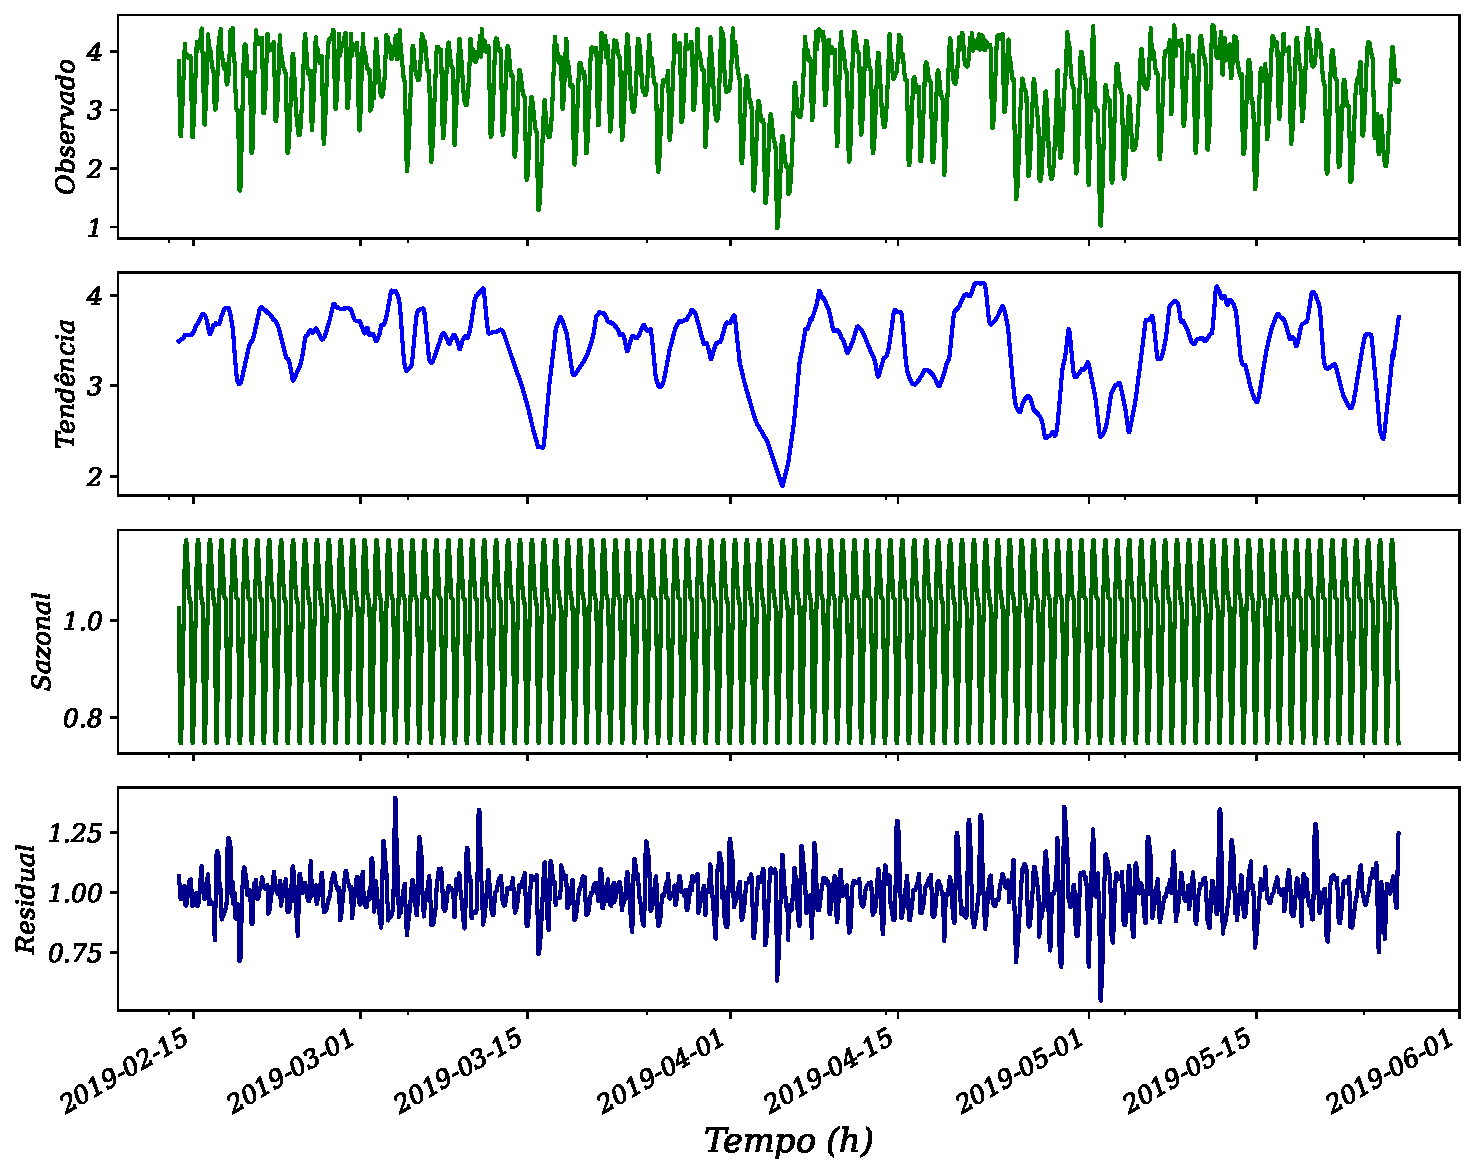
\includegraphics[width=\linewidth]{Resultados/Figuras/STL}	
\end{figure}


Essa decomposição divide os dados em sazonalidade, para descobrir no modelo ARIMA e seus antecessores que os dados podem ser coletados por hora, dia, mês ou ano. Saber que uma série tem sazonalidade torna o modelo ARIMA mais robusto, permitindo o uso do modelo ARIMA com sazonalidade, conhecido como SARIMA. Esses dados, por representarem uma sazonalidade difícil de ser notada, resultam em modelos com essa sazonalidade que não apresentam muita redução nos valores dos erros.

A tendência dos dados reflete como a série se comporta ao longo prazo, se ela pode subir ou reduzir o padrão. Tanto uma série pode ser estacionária ou não estacionária. Pela Figura \ref{fig:stl}, a tendência parece ser linear, caracterizando a série como estacionária. No entanto, essa série não possui um padrão sazonal, o que faz com que os modelos de ARIMA com sazonalidade apresentem erros maiores em comparação aos modelos clássicos.

O resíduo nos dados da série temporal é uma forma de avaliar que a série trabalhada possui várias irregularidades, levando aos resíduos que ajudam a verificar a verdadeira essência dos dados. Como esses dados foi coletado por hora ele tem muita oscilação, trazendo muitos ruídos ao longo da análise.

A Figura \ref{fig:person} mostra a correlação de Pearson entre as variáveis do conjunto de dados deste estudo. Essa figura representa a matriz (simétrica) da dependência/correlação entre as variáveis. Analisamos as correlações das variáveis de entrada com a variável de saída. Serão descartadas as variáveis com correlação menor que 5\% e maior que 90\%.

\begin{figure}[!htb]
	\centering
	\caption{Correlação de Pearson.}
	\label{fig:person}	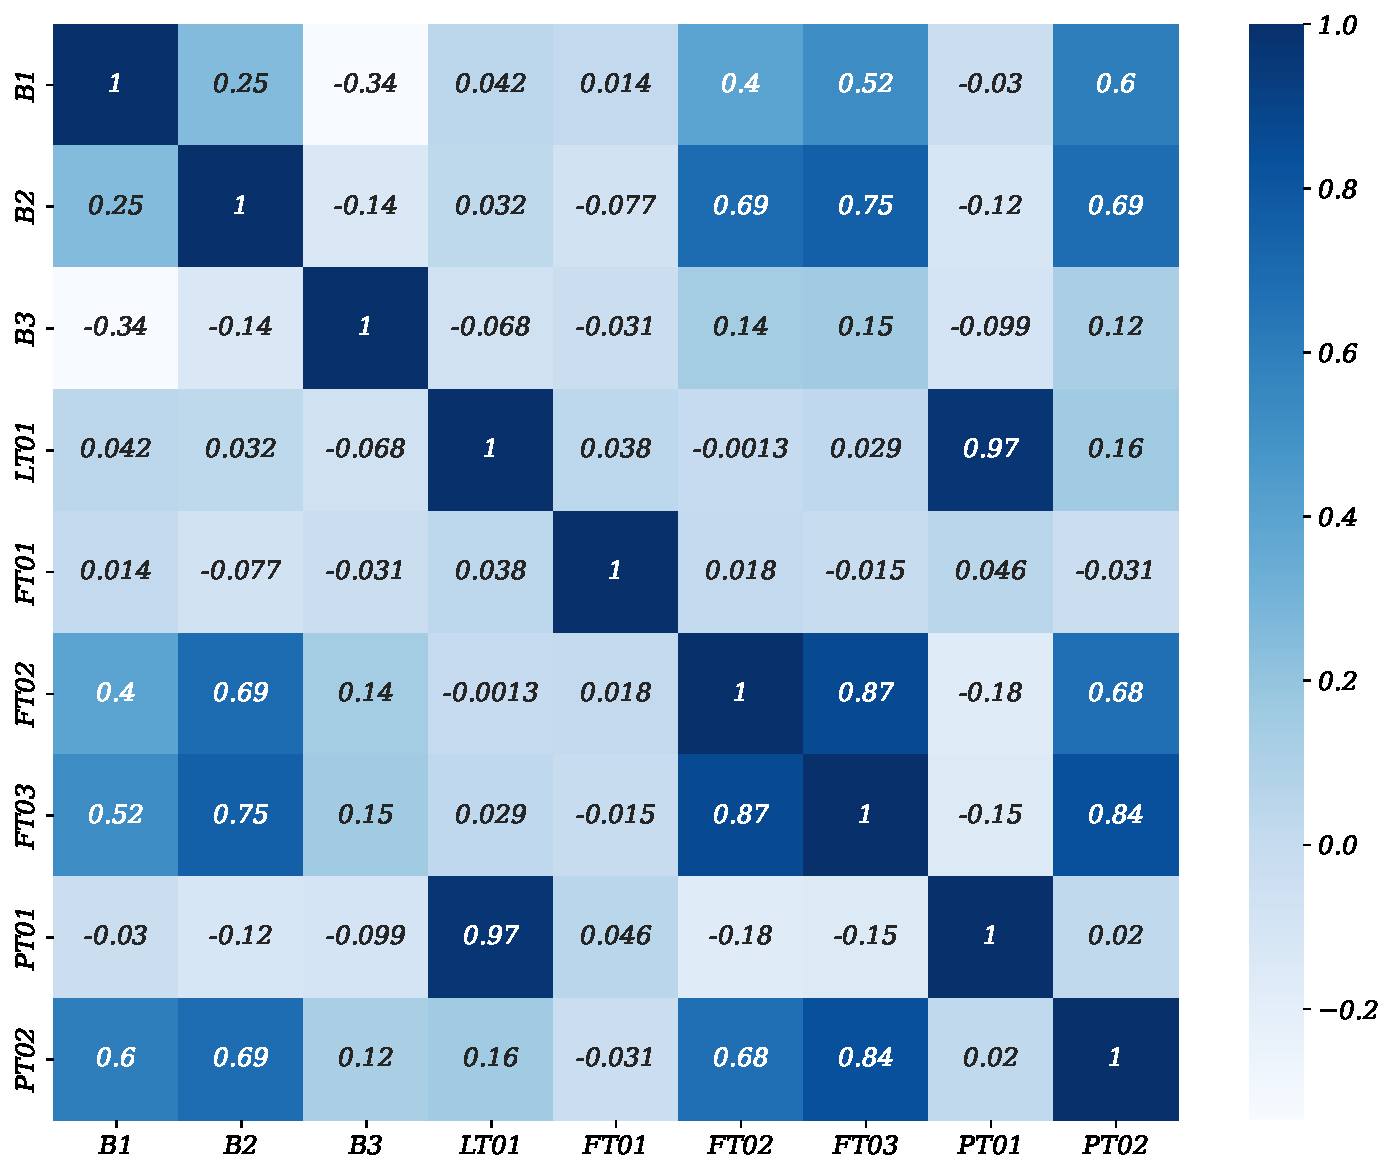
\includegraphics[width=0.7\linewidth]{Resultados/Figuras/person}
		
\end{figure}

No contexto das análises de dados, várias técnicas de EDA têm sido adotadas. Neste estudo, são realizadas diversas análises, incluindo a correlação de Pearson, para identificar quais variáveis podem ser excluídas devido a ruídos (correlação baixa) ou por estarem altamente correlacionadas com a variável de saída do estudo, que é a variável LT01, representando o nível do tanque de armazenamento d'água pela SANEPAR no Bairro Alto. As variáveis removidas têm pouca correlação com a LT01; por exemplo, as variáveis B3 e FT02 apresentam correlação baixa e serão excluídas.

O termo ``correlação baixa'' indica que há pouca relação linear entre as variáveis, sugerindo uma associação fraca entre elas. Um teste de hipótese é comumente usado para determinar se essa correlação é estatisticamente significativa. Nos testes de correlação de Pearson, se o valor-p for menor que um determinado nível de significância (como $0,05$), então a correlação é considerada estatisticamente significativa.

Nesse conjunto de dados que está sendo trabalhado, há uma forte correlação da variável PT01 com o LT01 conforme visto na Figura \ref{fig:lr-lt01-m3} que fornece uma representação dos coeficientes $\beta_0$ e $\beta_1$, que são os coeficientes da correlação linear entre as variáveis. Um aumento de $1$ na variável $x$ está associado a um aumento proporcional de $\beta_1$ na variável $y$. O valor de $\beta_0$ representa o valor de $y$ quando $x$ é igual a $0$.

\begin{figure}[!htb]
	\centering
	\caption{Relação entre LT01 e PT01 cuja correlação de Pearson é 97\%.}
	\label{fig:lr-lt01-m3}
	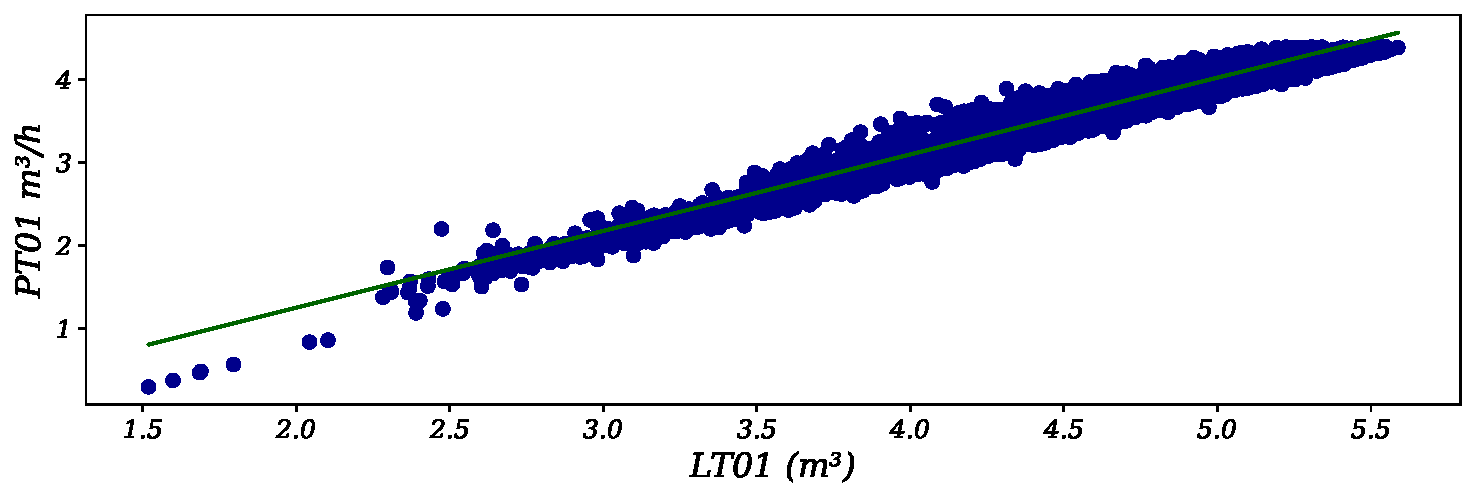
\includegraphics[width=0.7\linewidth]{Resultados/Figuras/LR}
\end{figure}


Na Figura \ref{fig:acfa}, observa-se a distinção entre ACF, apresentada na Figura \ref{fig:acfa}, e PACF, mostrada na Figura \ref{fig:pacf}. A autocorrelação é uma métrica que indica a relação entre os valores de uma série temporal em diferentes defasagens, capturando tanto correlações diretas quanto indiretas. Por sua vez, a autocorrelação parcial mensura apenas a correlação direta entre os valores, ignorando a influência de defasagens intermediárias. Essas análises são cruciais para detectar padrões e dependências entre os valores da série temporal, o que é essencial para a modelagem e previsão desses dados.

O intervalo de confiança padrão de $95\%$, destacado pela faixa azul nas Figuras \ref{fig:acfa} e \ref{fig:pacf}, serve como referência crítica. Observações fora desse intervalo indicam correlações estatisticamente significativas, sugerindo a presença de padrões ou estrutura na série temporal.


\begin{figure}[!htb]
	\centering
	\caption{Autocorrelação.}\label{fig:acfa}	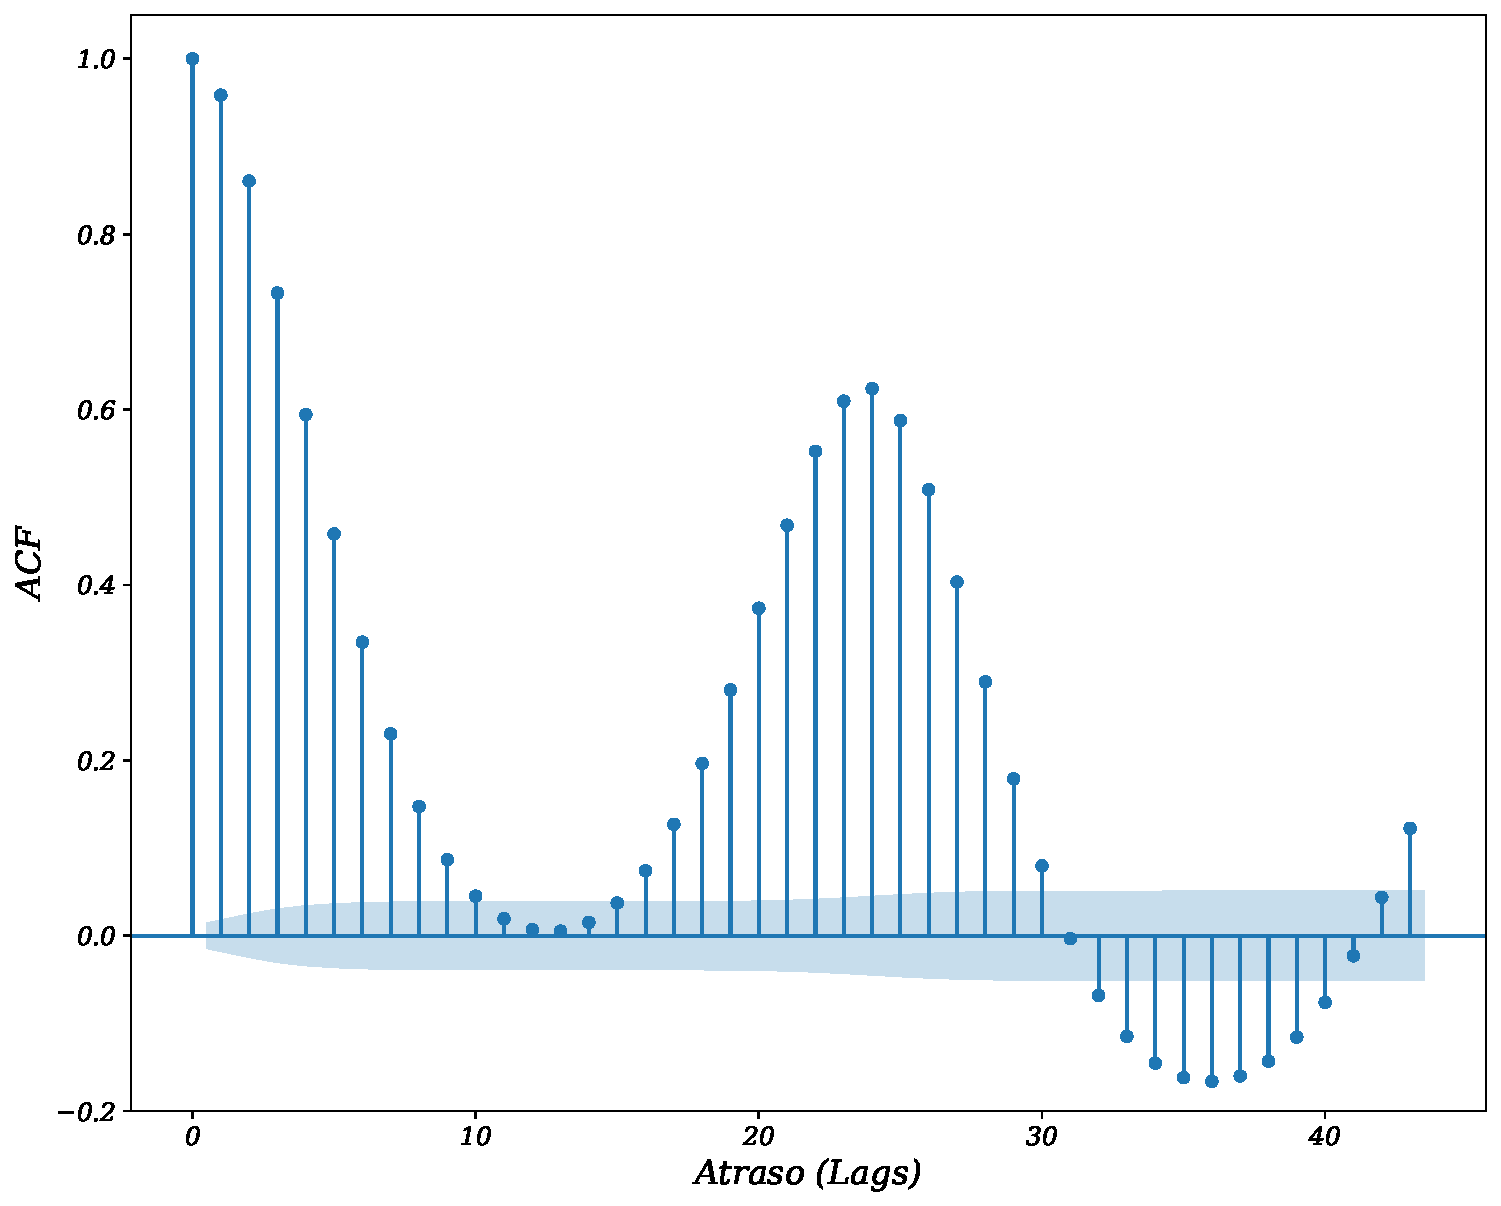
\includegraphics[width=0.6\linewidth]{Resultados/Figuras/acf} 
\end{figure}

\begin{figure}[!htb]
	\centering
	\caption{Autocorrelação parcial.}\label{fig:pacf}	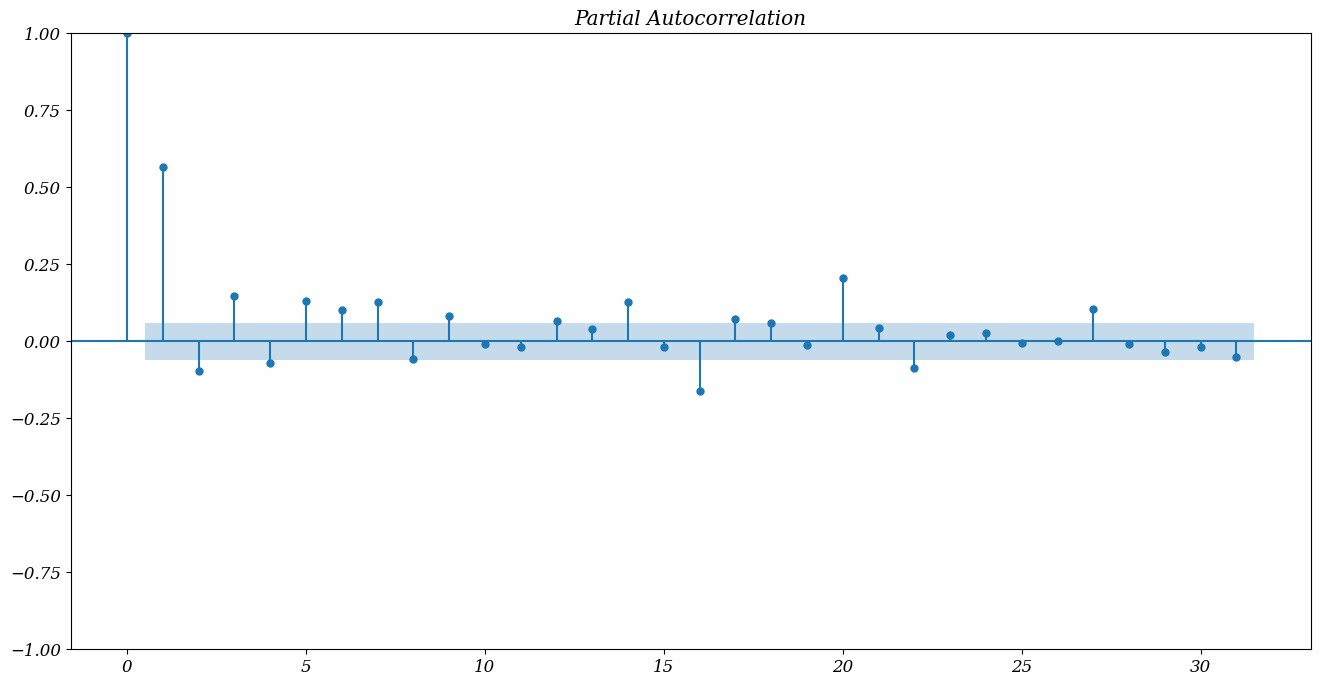
\includegraphics[width=0.6\linewidth]{Resultados/Figuras/pacf}
\end{figure}


A correlação visualizada na Figura \ref{fig:acfa} é fundamental para a interpretação do teste ADF. Em uma série de ruído branco, os valores são completamente aleatórios e não apresentam correlação significativa. Portanto, quando há correlação presente na série, isso indica a existência de padrões ou dependências entre os valores, o que pode ser explorado para a modelagem e previsão da série temporal.

Demonstrar que uma série temporal tem ou pode ter um ruído branco também é conveniente para a análise da EDA.
Na Figura \ref{fig:ruido-branco}, é possível observar uma série temporal que pode ser caracterizada como ruído branco, se suas variáveis forem independentes e distribuídas de forma idêntica, com média zero. Isso implica que todas as variáveis possuem a mesma variância ($\sigma^2$) e que cada valor não possui correlação com os demais valores da série.

\begin{figure}[!htb]
	\centering
	\caption{Ruído branco.}
	\label{fig:ruido-branco}
	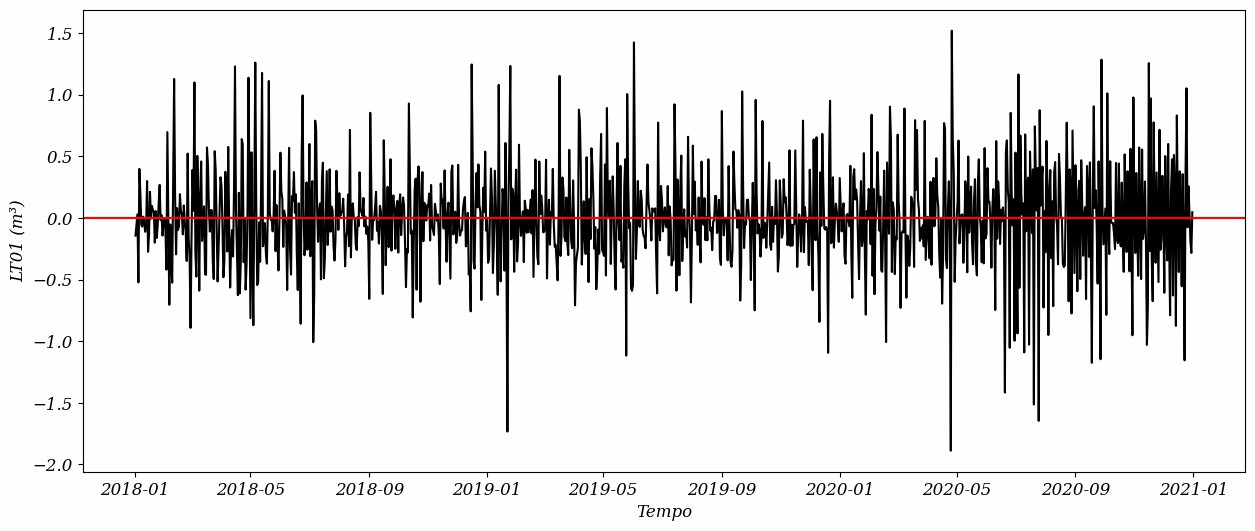
\includegraphics[width=0.7\linewidth]{Resultados/Figuras/ruido-branco}
\end{figure}


ADF de $-12,515$ indica a evidência de estacionariedade na série temporal do nível do tanque LT01. 
O valor de p expresso como $2,62\times 10^{-23}$ está associado ao teste ADF. No contexto do teste ADF, a hipótese nula é a presença de raiz unitária na série temporal, indicando não estacionariedade. Dado o valor de p de $2,62\times 10^{-23}$, evidencia-se uma probabilidade muito baixa, indicando forte suporte contra a hipótese nula e sugerindo que a série temporal é estacionária. Na Tabela \ref{tb:adf}, são apresentados todos os dados do teste para estacionariedade.Os resultados indicam fortes evidências contra a hipótese nula. Com um teste ADF de $-12,515 $ e um valor de p extremamente baixo de $2,62 \times 10^{-23}$, rejeita-se a hipótese nula de presença de raiz unitária. Os $44$ atrasos utilizados e as $17.477$ observações corroboram a análise estatística. Ao comparar a estatística de teste ADF com os valores críticos, observa-se que está significativamente abaixo deles em todos os níveis de significância $(1\%, 5\%, 10\%)$. Portanto, a conclusão é de que os dados não possuem raiz unitária, indicando que são estacionários.

\begin{table}[!htb]
	\centering
	\caption{Teste ADF.}\label{tb:adf}
	\begin{tabular}{ll}
		\hline
		Valor de p & $2,62 \times 10^{-23}$ \\
		Atrasos utilizados & $44$ \\
		Número de observações & $17.477$ \\
		Valor crítico $(1\%)$ & $-3,431$ \\
		Valor crítico $(5\%)$ & $-2,862$ \\
		Valor crítico $(10\%)$ & $-2,567$ \\
		\hline
	\end{tabular}
\end{table}

Para a previsão os dados foram divididos em conjuntos de treinamento, validação, e teste \cite{raschka2015practical, geron2017hands_on}. Quanto à divisão dos dados, foi adotada uma estratégia básica em que $70\%$ dos dados foram destinados ao conjunto de treinamento e $30\%$ restantes foram reservados para o conjunto de teste. Dentro dos $70\%$ de treinamento, foi realizada uma subdivisão em que $80\%$ desses dados foram usados novamente para treinamento e os $20\%$ restantes foram utilizados para validação. 

A estratégia recursiva é mencionada por \citeonline{PETROPOULOS2022705} como uma abordagem eficaz na previsão de séries temporais de múltiplos passos. De acordo com o autor, essa estratégia envolve o uso de previsões anteriores como entradas para prever os próximos passos da série temporal. A abordagem recursiva tem demonstrado potencial para melhorar a acurácia das previsões de séries temporais de longo prazo.


\noindent\textbf{Modelos de Séries Temporais} (\textbf{AR}, \textbf{ARIMA}, \textbf{ARIMAX}, \textbf{ARMA}, \textbf{ARX}, \textbf{MA}, \textbf{SARIMA}, \textbf{SARIMAX}, \textbf{Prophet}):

Para todos os modelos dessa categoria, as características de entrada e variáveis exógenas são semelhantes. Ele utiliza apenas o histórico de dados do LT01 como entrada e considera outras variáveis, como FT01, FT03, PT01, PT02, B1 e B2, como variáveis exógenas. A configuração consiste em organizar os dados históricos do nível do reservatório em séries temporais e ajustar cada modelo de acordo com sua técnica específica para prever valores futuros com base nos padrões identificados nos dados históricos do LT01.

\noindent\textbf{Redes Neurais Recorrentes} (\textbf{RNN}, \textbf{LSTM}, \textbf{GRU}):

Assim como nos modelos de séries temporais, as entradas e variáveis exógenas dessas redes neurais são as mesmas mencionadas anteriormente. Ele também utiliza apenas o histórico de dados do LT01 como entrada e considera outras variáveis como exógenas. No entanto, a configuração difere, pois os dados históricos do nível do reservatório são organizados em sequências temporais, e a rede é treinada com camadas recorrentes para aprender padrões temporais e fazer previsões futuras.

\noindent\textbf{Outros Modelos} (\textbf{CNN}, \textbf{MLP}, \textbf{DT}, \textbf{RF}, \textbf{XGBoost}, \textbf{LightGBM}):

Similarmente aos modelos anteriores, esses modelos também compartilham as mesmas entradas e variáveis exógenas. Ele utiliza apenas o histórico de dados do LT01 como entrada e considera outras variáveis como exógenas. A configuração, no entanto, varia dependendo do modelo. Os dados históricos do nível do reservatório são organizados em conjuntos de treinamento para cada modelo, e cada um é treinado para aprender padrões nos dados e fazer previsões futuras. Uma exceção é o modelo DT, que utiliza o LT01 para previsão e o PT01 como variável alvo no eixo $y$.


O MISO foi o modelo usado neste estudo. O modelo ARIMA, juntamente com suas variantes e extensões, foi amplamente estudado durante a pesquisa, assim como modelos regressivos que envolvem múltiplas variáveis de entrada e uma variável de saída, neste caso, a LT01. As demais variáveis, como FT01, FT03, PT01, PT02, B1 e B2, foram utilizadas como suporte para melhorar o modelo do tipo ARIMAX, modelos com variáveis exógenas.

Quando aplicado sem o uso de variáveis exógenas, o modelo ARIMA apresenta apenas uma entrada, semelhante ao modelo de regressão linear. No entanto, ao incluir variáveis exógenas, o modelo se torna MISO, permitindo uma modelagem  abrangente e considerando a correlação das várias para prever a variável de interesse, LT01.

A previsão dos dados foi feita com diferentes horizontes de previsão como $1$ hora, $6$ horas, $12$ horas, e $24$ horas. Essas estratégias de previsão permitem a comparação entre os modelos de regressão e modelos ARIMA em diferentes horizontes temporais.

Além desses modelos de previsão, vários outros modelos foram utilizados no estudo, tais como DT, RF, XGBoost, LightGBM, MLP, LSTM, GRU, Prophet, RNN, e CNN, a fim de obter o melhor resultado para a previsão de séries temporais de abastecimento d'água.


Na Tabela \ref{tab:autoarima_params} são exibidos todos os valores obtidos pela biblioteca do \textit{Python} autoARIMA, resultantes para $p$, que representa a ordem do componente AR; $d$, que indica o número de diferenciações não sazonais; $q$, que denota a ordem do componente MA; $P$, que corresponde à ordem do componente AR sazonal; $D$, que representa o número de diferenciações sazonais; $Q$, que indica a ordem do componente MA sazonal; e $M$, que representa o período sazonal (o número de observações em um ciclo sazonal).


\begin{table}[!htb]
	\centering
	\caption{Parâmetros para os modelos ARIMA utilizando a função autoARIMA.}
	\label{tab:autoarima_params}
	\small
	\begin{tabular}{ll}
	\toprule
	\text{Modelos} & \text{Parâmetros}   \\
	\midrule
		AR(p) & $ p = 3 $  \\
		ARX(p) & $ p = 3 $ \\
		MA(q) & $ q = 3 $   \\
		ARMA(p, q) & $ p = 3 $, $ q = 3 $  \\
		ARIMA(p, d, q) & $ p = 3 $, $ d = 1 $, $ q = 3 $  \\
		ARIMAX(p, d, q) & $ p = 3 $, $ d = 1 $, $ q = 3 $  \\
		SARIMA(p, d, q)(P, D, Q) & $ p = 3 $, $ d = 1 $, $ q = 3 $, $ P = 0 $, $ D = 1 $, $ Q = 2 $ \\
		SARIMAX(p, d, q)(P, D, Q, M) & $ p = 3 $, $ d = 1 $, $ q = 3 $, $ P = 0 $, $ D = 1 $, $ Q = 2 $, $ M = 4 $\\
		\bottomrule
	\end{tabular}
\end{table}

Os hiperparâmetros dos modelos foram otimizados usando a biblioteca Optuna do \textit{Python}. Nesse contexto, foram empregadas técnicas bayesianas, especificamente o algoritmo TPE visando uma otimização mais eficiente.

Na Tabela \ref{tab:hiperparametros} são descritos os hiperparâmetros dos modelos XGBoost, LightGBM, RF, e DT, onde NE é o número de estimadores, PM é a profundidade máxima, MAD é o mínimo de amostras por divisão, MAF é o mínimo de amostras por folha, e TA é a taxa de aprendizado. 

\begin{table}[!htb]
	\centering
	\caption{Hiperparâmetros otimizados dos modelos.}
	\label{tab:hiperparametros}
	\begin{tabular}{llllll}
		\toprule
		\text{Modelo} & \text{Estimadores} & \text{PM} & \text{MAD} & \text{MAF} & \text{TA} \\
		\midrule
			DT & N/A & 976 & 14 & 14 & N/A \\
			LightGBM & 419 & 18 & 8 & 13 & 0,021 \\
			RF & 477 & 18 & 4 & 11 & N/A \\
			XGBoost & 1752 & 4 & 23 & 24  & 0,014 \\	
		\bottomrule
	\end{tabular}
\end{table}


Os hiperparâmetros dos modelos de rede neural artificial (RNA), como RNN, MLP, CNN, GRU e LSTM, obtidos através da otimização TPE da biblioteca Optuna em Python, são exibidos na Tabela \ref{tab:hyperparameters_summary}. CNN utilizou um kernel de tamanho 5 e uma camada densa, enquanto MLP utilizou uma única camada densa.

\begin{table}[!htb]
	\centering
	\caption{Hiperparâmetros otimizados para RNA.}
	\label{tab:hyperparameters_summary}
	\small
	\begin{tabular}{lllll}
		\toprule
		\text{Modelo} & \text{Layers} & \text{Tamanho} & \text{No. Épocas} & \text{Dropout/} \\
		&&\text{do Batch}&& \text{Learning Rate}\\
		\midrule
		CNN & 4 & 13 & 100 & 0,24; 0,00067 \\
		GRU & 2 & 16 & 69 & -- ; 0,01  \\
		LSTM & 4 & 32 & 122 & 0,2 ; 0,01 \\
		MLP & 3 & 32 & 65 & 0,218, 0,00030 \\
		RNN & 4 & 16 & 50 & 0,2 ; 0,01 \\
		\bottomrule
	\end{tabular}
\end{table}



\subsection{Aplicando os Modelos de Previs\~ao}

Na análise dos modelos desenvolvidos, observou-se que o modelo DT obteve o melhor desempenho, tanto para previsões de curto prazo, durante as horas de pico entre 18h e 21h, quanto para outros períodos. Além disso, o Prophet foi o segundo modelo que mais apresento resultados satisfatório em previsão de longo prazo.

Uma observação recorrente foi a superioridade dos modelos que incorporam variáveis exógenas em termos de capacidade de previsão, evidenciada nas Figuras \ref{fig:1-ar-arx-ma} a \ref{fig:prophet1} e nas Tabelas \ref{tb:apd-trn} a \ref{tb:apd-int}, onde os valores menores foram destacados em \textbf{negrito}. O modelo DT destacou-se como o melhor em termos de eficácia nas previsões realizadas, seguido pelo modelo Prophet. Desde a \ref{fig:1-ar-arx-ma} a \ref{fig:prophet1} são ilustrados cenários distintos de previsão e comparação entre os modelos DT e Prophet, respectivamente, sendo o primeiro a escolha mais adequada. As Figuras são exibidas com um corte temporal da data 2019/12/01, 2020/01/02.


\begin{figure}[!htb]
	\centering
	\caption{Comparação dos modelos de previsão AR, ARX, MA e ARMA 24 passo à frente.}
	\label{fig:1-ar-arx-ma}
	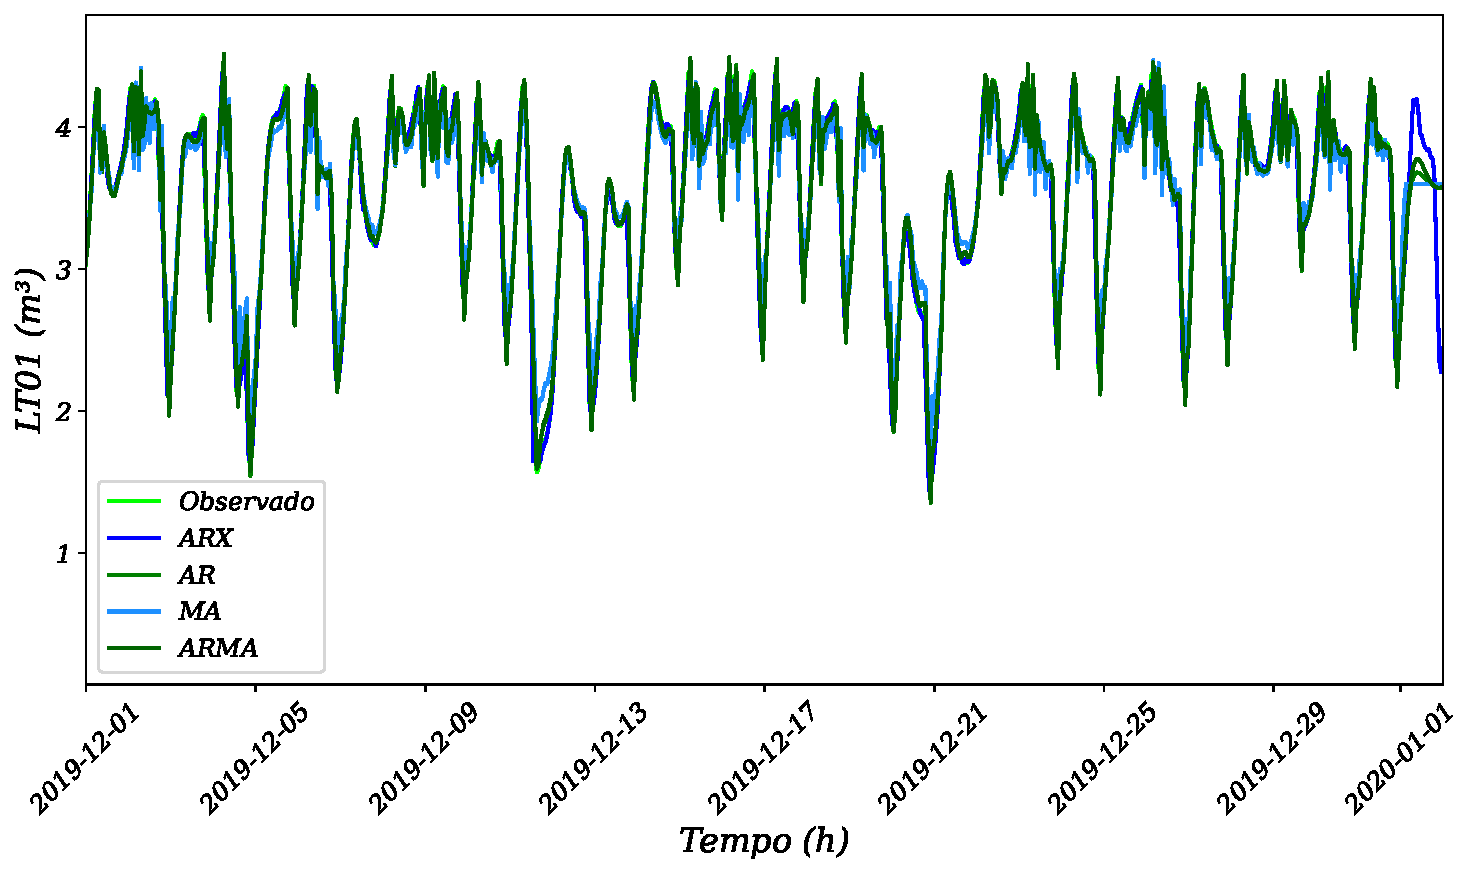
\includegraphics[width=0.7\linewidth]{Resultados/Figuras/ARX-AR-MA-ARMA-24}
	
\end{figure}
\begin{figure}[!htb]
	\centering
	\caption{Comparação dos modelos de previsão ARIMA, ARIMAX, SARIMA e SARIMAX 24 passo à frente.}
	\label{fig:1-arimax-sarima-sarimax}
	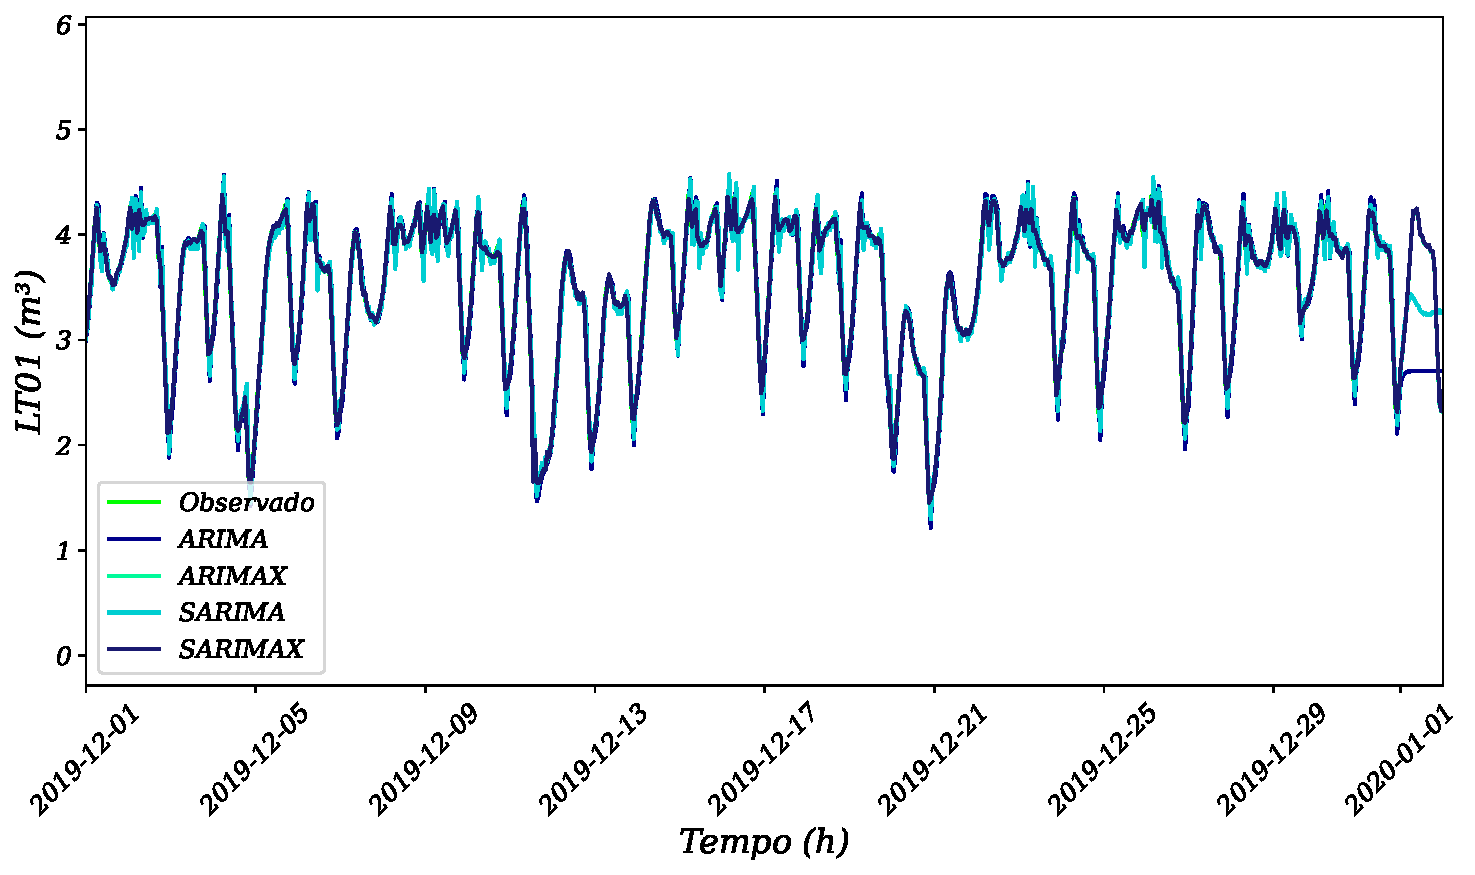
\includegraphics[width=0.7\linewidth]{Resultados/Figuras/ARIMA-SARIMA-ARIMAX-SARIMAX-24}
	
\end{figure}

\begin{figure}[!htb]
	\centering
	\caption{Comparação dos modelos DT, RF, XGBoost e LightGBM 1 passo à frente.}
	\label{fig:lr-xgb-lgbm-rf}
	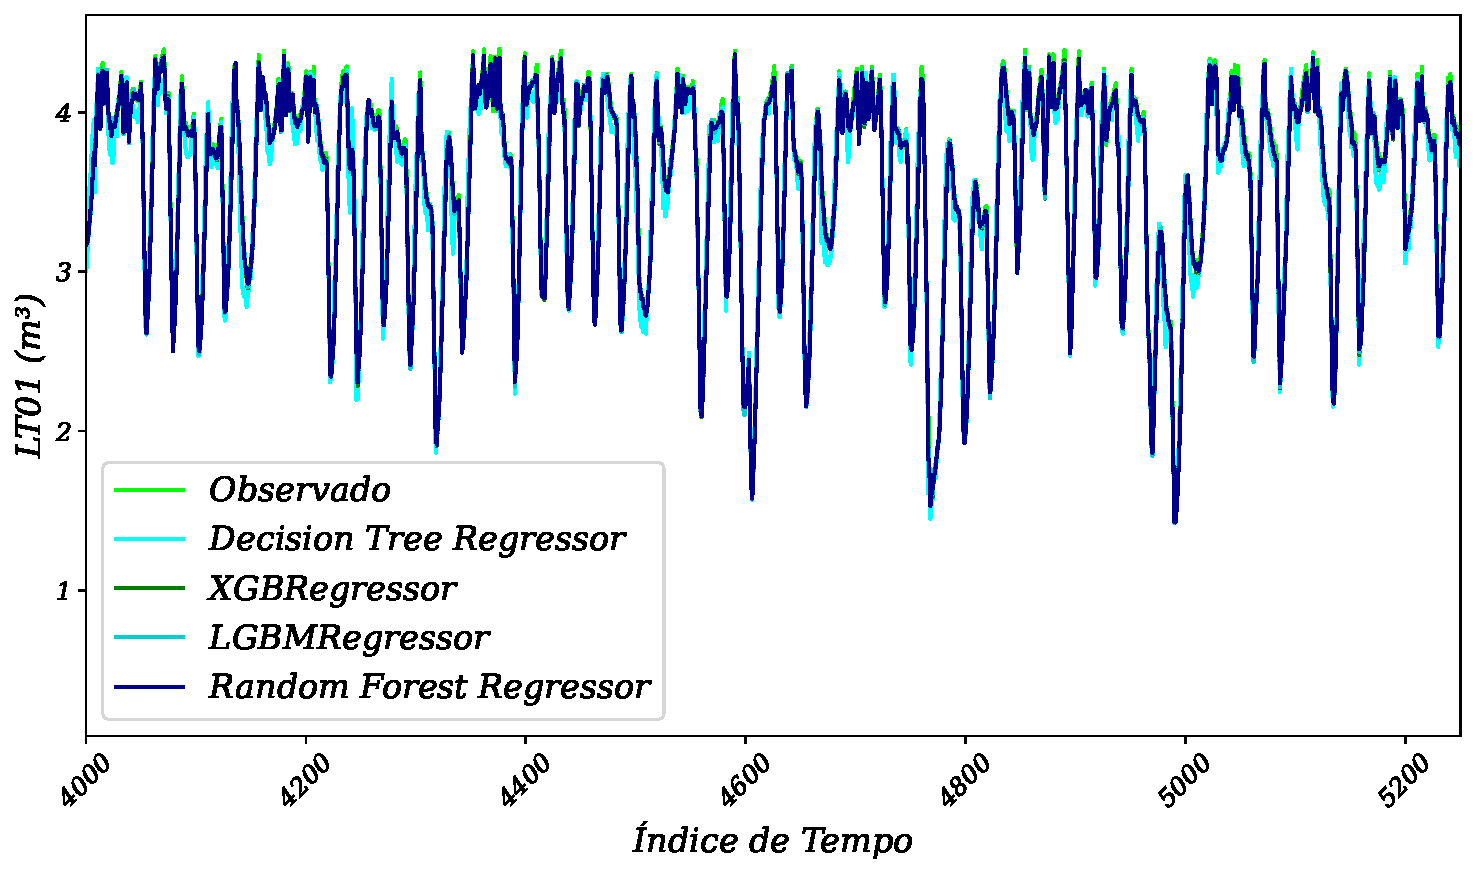
\includegraphics[width=0.7\linewidth]{Resultados/Figuras/LR-XGB-LGBM-RF}
	
\end{figure}

\begin{figure}[!htb]
	\centering
	\caption{Modelo de previsão GRU para vários horizontes de previsão.}
	\label{fig:gru1}
	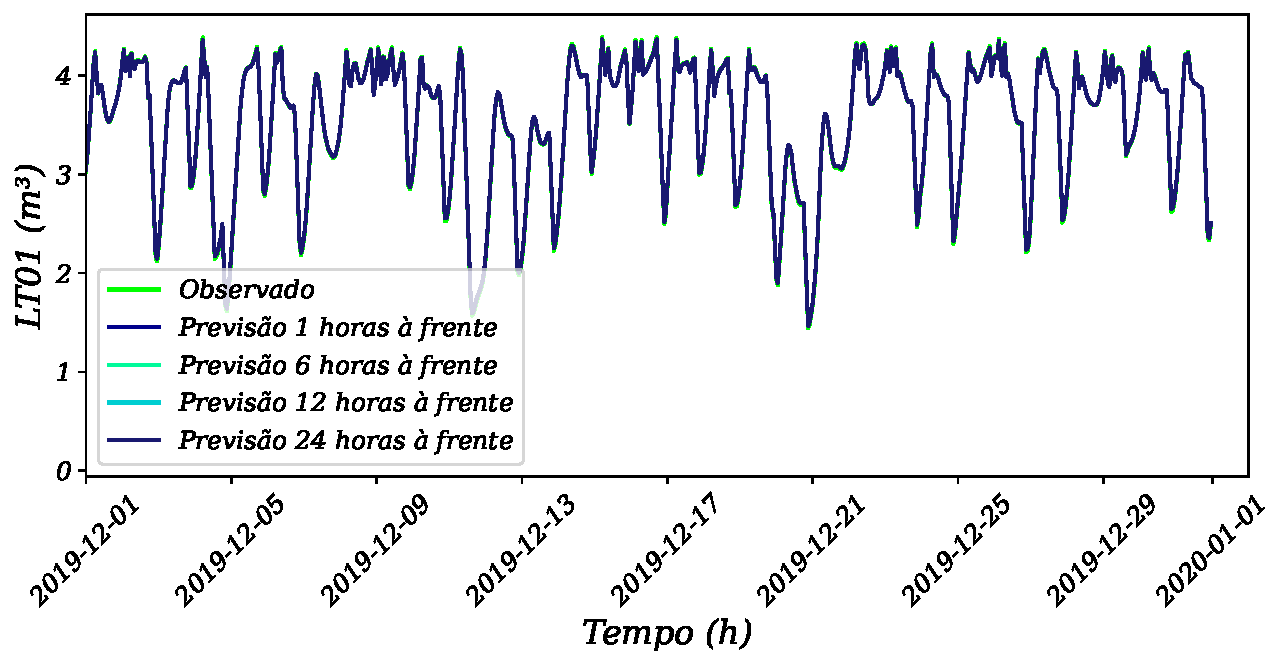
\includegraphics[width=0.7\linewidth]{Resultados/Figuras/GRU}
	
\end{figure}

\begin{figure}[!htb]
	\centering
	\caption{Modelo de previsão LSTM para vários horizontes de previsão.}
	\label{fig:lstm}
	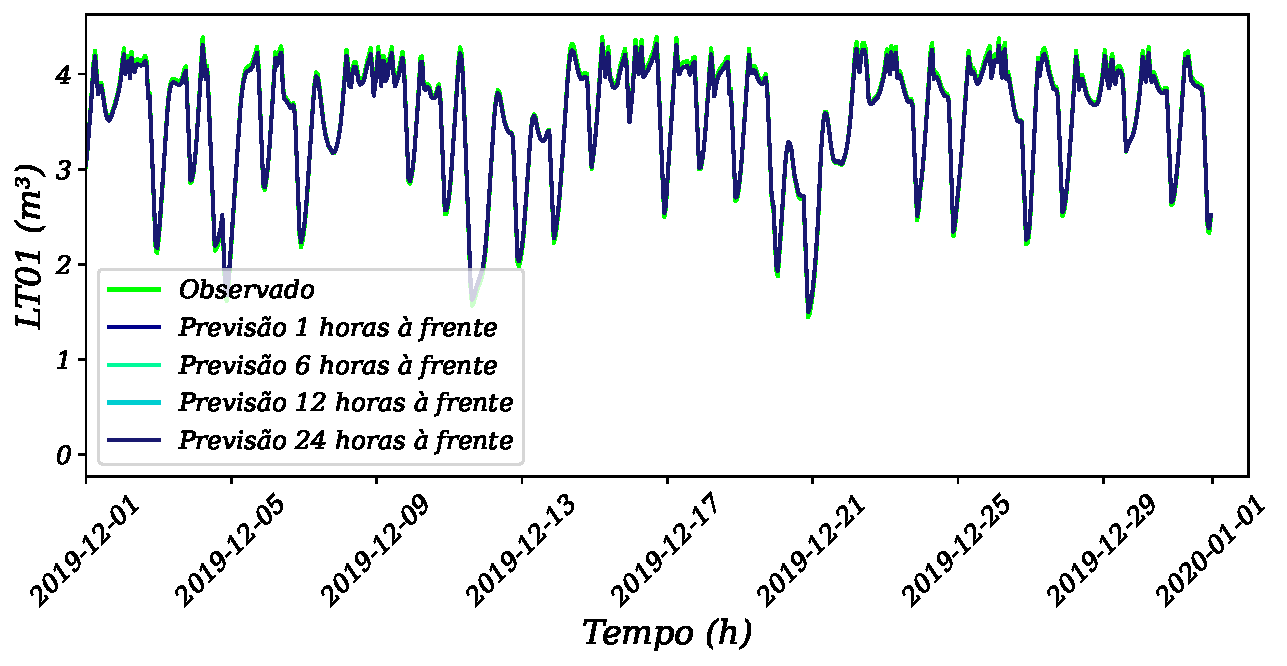
\includegraphics[width=0.7\linewidth]{Resultados/Figuras/LSTM}
	
\end{figure}

\begin{figure}[!htb]
	\centering
	\caption{Modelo de previsão RNN para vários horizontes de previsão.}
	\label{fig:rnn}
	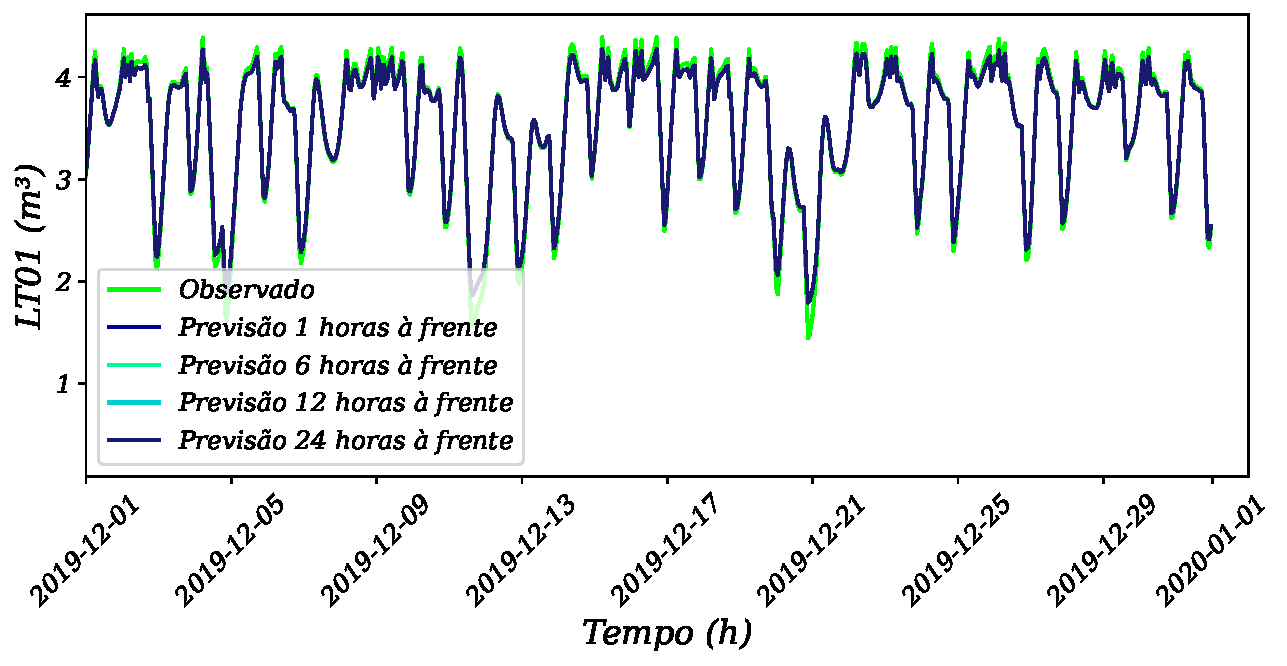
\includegraphics[width=0.7\linewidth]{Resultados/Figuras/RNN}
\end{figure}
\begin{figure}[!htb]
	\centering
	\caption{Previsões do modelo Prophet para vários horizontes de previsão.}\label{fig:prophet1}
	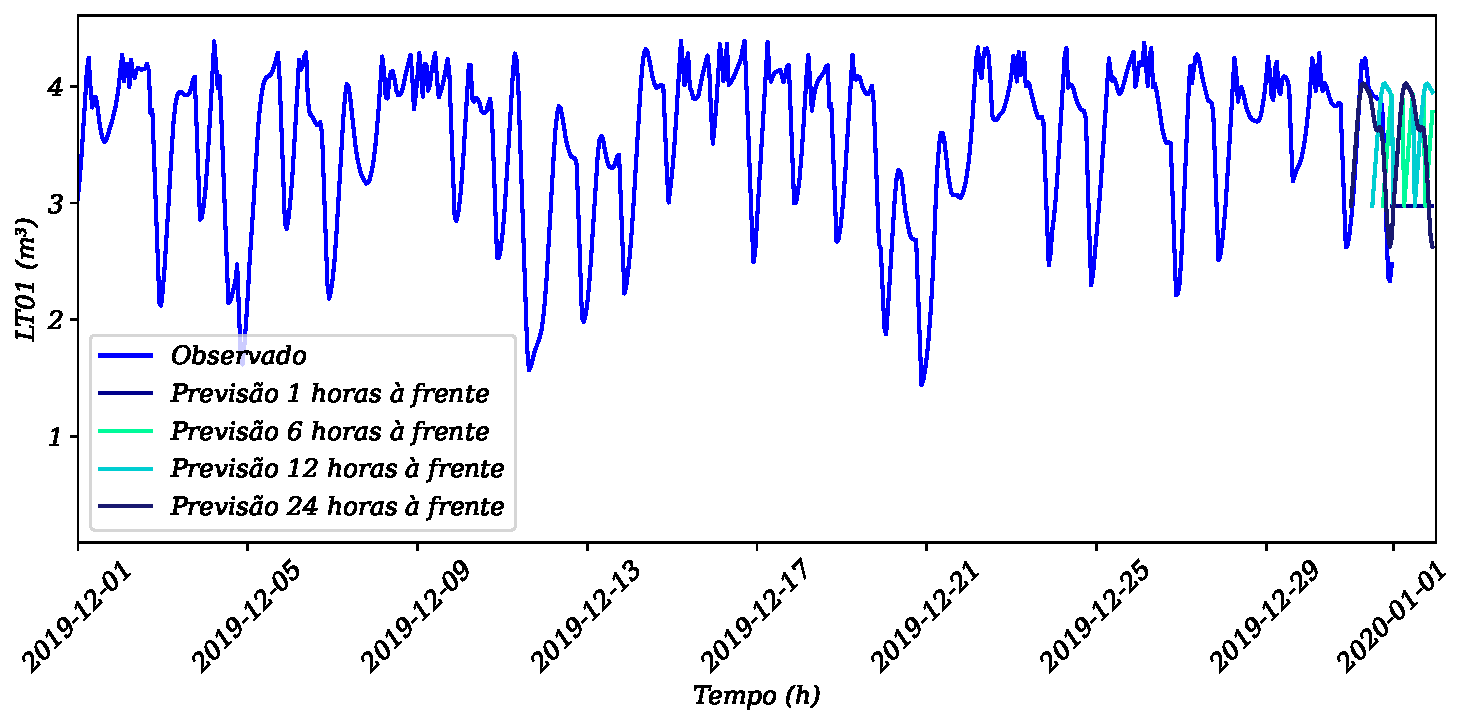
\includegraphics[width=0.7\linewidth]{Resultados/Figuras/prophet}	
\end{figure}




\begin{landscape}
\begin{table}[!htb]
	\centering
	\setlength{\tabcolsep}{2pt} % Reduzir o espaçamento entre as colunas
	\caption{Comparação dos modelos de previsão através das métricas de desempenho para dados de treino.}\label{tb:apd-trn}
\begin{tabular}{llllllllllllllllllll}
\toprule
Horizontes                         & Métricas & A     & B     & C     & D     & E     & F     & G              & H      & I     & J     & K     & L     & M     & N     & O     & P     & Q     & R     \\ \midrule
\multirow{3}{*}{1 hora à frente}   & SMAPE (\%)    & 7,81  & 7,85  & 7,83  & 7,79  & 8,01  & 18,77 & \textbf{7,69}  & 35,89  & 24,60 & 18,55 & 8,37  & 18,77 & 21,27 & 18,38 & 23,36 & 8,03  & 7,79  & 19,56 \\
& MAE      & 0,25  & 0,25  & 0,25  & 0,25  & 0,25  & 0,10  & 0,35           & 1,44   & 0,93  & 0,65  & 0,27  & 0,10  & 0,77  & 0,64  & 0,87  & 0,26  & 0,25  & 0,69  \\
& RRMSE (\%)    & 0,09  & 0,09  & 0,10  & 0,09  & 0,10  & 0,42  & 0,21           & 0,65   & 1,36  & 0,21  & 0,10  & 0,42  & 0,77  & 0,21  & 1,28  & 0,10  & 0,10  & 0,22  \\ \hline
\multirow{3}{*}{6 horas à frente}  & SMAPE (\%)    & 19,99 & 19,93 & 20,10 & 20,01 & 20,08 & 20,37 & \textbf{13,94} & 83,75  & 58,21 & 18,55 & 18,34 & 20,37 & 33,71 & 24,25 & 50,20 & 20,12 & 20,13 & 26,23 \\
& MAE      & 0,64  & 0,64  & 0,64  & 0,64  & 0,64  & 0,20  & 0,59           & 4,94   & 2,77  & 0,65  & 0,60  & 0,20  & 1,12  & 0,88  & 2,25  & 0,64  & 0,64  & 0,97  \\
& RRMSE (\%)    & 0,23  & 0,23  & 0,23  & 0,23  & 0,23  & 0,44  & \textbf{0,16}  & 1,70   & 4,15  & 0,21  & 0,21  & 0,44  & 1,15  & 0,32  & 3,42  & 0,23  & 0,23  & 0,34  \\ \hline
\multirow{3}{*}{12 horas à frente} & SMAPE (\%)    & 23,23 & 23,03 & 23,31 & 23,23 & 23,14 & 19,04 & \textbf{13,94} & 98,06  & 60,06 & 18,55 & 21,31 & 19,04 & 24,62 & 24,22 & 51,28 & 23,37 & 23,38 & 26,26 \\
& MAE      & 0,75  & 0,75  & 0,75  & 0,75  & 0,75  & 0,12  & 0,59           & 6,62   & 2,91  & 0,65  & 0,70  & 0,12  & 0,83  & 0,88  & 2,32  & 0,76  & 0,76  & 0,97  \\
& RRMSE (\%)    & 0,27  & 0,26  & 0,27  & 0,27  & 0,26  & 0,42  & \textbf{0,16}  & 2,23   & 4,36  & 0,21  & 0,25  & 0,42  & 0,91  & 0,32  & 3,53  & 0,27  & 0,27  & 0,34  \\ \hline
\multirow{3}{*}{24 horas à frente} & SMAPE (\%)    & 13,53 & 13,37 & 13,69 & 13,53 & 13,70 & 19,63 & 13,94          & 104,82 & 60,10 & 18,55 & 12,90 & 19,63 & 6,55  & 24,25 & 51,13 & 13,77 & 13,70 & 26,75 \\
& MAE      & 0,43  & 0,43  & 0,44  & 0,43  & 0,44  & 0,16  & 0,59           & 7,59   & 2,91  & 0,65  & 0,42  & 0,16  & 0,23  & 0,88  & 2,31  & 0,44  & 0,44  & 1,00  \\
& RRMSE (\%)    & 0,17  & 0,17  & 0,17  & 0,17  & 0,17  & 0,43  & 0,16           & 2,53   & 4,37  & 0,21  & 0,16  & 0,43  & 0,29  & 0,32  & 3,52  & 0,17  & 0,17  & 0,35  \\ \cmidrule(l){1-20} 

\end{tabular}
	
	\captionsetup{justification=centering} % Centralizar a legenda
	A -- AR,
	B -- ARIMA,
	C -- ARIMAX,
	D -- ARMA,
	E -- ARX,
	F -- CNN,
	\textbf{G -- DT},
	H -- GRU,
	I -- LSTM,
	J -- LigthGBM,
	K -- MA,
	L -- MLP,
	M -- Prophet,
	N -- RF,
	O -- RNN,
	P -- SARIMA,
	Q -- SARIMAX,
	R -- XGBoost
	

\end{table}

	\newpage

\begin{table}[!htb]
	\centering
	\setlength{\tabcolsep}{2pt} % Reduzir o espaçamento entre as colunas
	\caption{Comparação dos modelos de previsão através das métricas de desempenho para dados de validação.}\label{tb:apd-vld}
	\begin{tabular}{llllllllllllllllllll}
		\toprule
		Horizontes                         & Métricas & A     & B             & C     & D     & E     & F     & G              & H      & I     & J     & K     & L     & M              & N     & O     & P     & Q     & R     \\ \midrule
		\multirow{3}{*}{1 hora à frente}   & SMAPE (\%)    & 7,88  & \textbf{7,66} & 8,31  & 7,87  & 8,29  & 20,52 & \textbf{8,51}  & 15,84  & 23,63 & 16,76 & 8,20  & 20,52 & 18,22          & 16,64 & 22,26 & 7,88  & 8,31  & 17,81 \\
		& MAE      & 0,26  & \textbf{0,25} & 0,27  & 0,26  & 0,27  & 1,88  & 0,39           & 0,54   & 0,92  & 0,60  & 0,27  & 1,88  & 0,50           & 0,60  & 0,86  & 0,26  & 0,27  & 0,65  \\
		& RRMSE (\%)    & 0,09  & \textbf{0,09} & 0,10  & 0,09  & 0,10  & 0,50  & 0,18           & 0,33   & 1,50  & 0,19  & 0,09  & 0,50  & 0,50           & 0,19  & 1,40  & 0,09  & 0,10  & 0,20  \\ \hline
		\multirow{3}{*}{6 horas à frente}  & SMAPE (\%)    & 19,39 & 19,92         & 19,91 & 19,47 & 19,89 & 18,90 & \textbf{12,66} & 72,77  & 55,41 & 16,76 & 17,81 & 18,90 & \textbf{29,73} & 21,03 & 47,27 & 19,32 & 19,89 & 22,81 \\
		& MAE      & 0,64  & 0,66          & 0,66  & 0,65  & 0,66  & 1,80  & \textbf{0,56}  & 4,04   & 2,68  & 0,60  & 0,60  & 1,80  & \textbf{0,93}  & 0,78  & 2,15  & 0,64  & 0,66  & 0,86  \\
		& RRMSE (\%)    & 0,23  & 0,23          & 0,23  & 0,23  & 0,23  & 0,48  & \textbf{0,14}  & 1,42   & 4,43  & 0,19  & 0,21  & 0,48  & 1,05           & 0,28  & 3,61  & 0,23  & 0,23  & 0,30  \\ \hline
		\multirow{3}{*}{12 horas à frente} & SMAPE (\%)    & 22,16 & 23,05         & 22,46 & 22,18 & 22,47 & 19,62 & \textbf{12,66} & 93,58  & 57,15 & 16,76 & 20,40 & 19,62 & 23,91          & 20,99 & 48,28 & 22,29 & 22,45 & 22,82 \\
		& MAE      & 0,74  & 0,77          & 0,75  & 0,74  & 0,75  & 1,83  & \textbf{0,56}  & 6,25   & 2,80  & 0,60  & 0,69  & 1,83  & \textbf{0,80}  & 0,78  & 2,22  & 0,75  & 0,75  & 0,86  \\
		& RRMSE (\%)    & 0,26  & 0,27          & 0,26  & 0,26  & 0,26  & 0,49  & \textbf{0,14}  & 2,09   & 4,64  & 0,19  & 0,24  & 0,49  & 0,97           & 0,28  & 3,72  & 0,26  & 0,26  & 0,29  \\ \hline
		\multirow{3}{*}{24 horas à frente} & SMAPE (\%)    & 12,32 & 12,85         & 12,70 & 12,29 & 12,70 & 17,69 & 12,66          & 102,11 & 57,20 & 16,76 & 11,65 & 17,69 & \textbf{5,05}  & 21,02 & 48,12 & 12,54 & 12,70 & 22,81 \\
		& MAE      & 0,41  & 0,42          & 0,42  & 0,40  & 0,41  & 1,74  & 0,56           & 7,42   & 2,81  & 0,60  & 0,39  & 1,74  & \textbf{0,17}  & 0,78  & 2,21  & 0,41  & 0,41  & 0,86  \\
		& RRMSE (\%)    & 0,16  & 0,17          & 0,16  & 0,16  & 0,16  & 0,46  & \textbf{0,14}  & 2,44   & 4,65  & 0,19  & 0,15  & 0,46  & 0,19           & 0,28  & 3,71  & 0,16  & 0,16  & 0,30  \\ \cmidrule(l){1-20} 	
	\end{tabular}
	
	
	\captionsetup{justification=centering} % Centralizar a legenda
	A -- AR,
	B -- ARIMA,
	C -- ARIMAX,
	D -- ARMA,
	E -- ARX,
	F -- CNN,
	\textbf{G -- DT},
	H -- GRU,
	I -- LSTM,
	J -- LigthGBM,
	K -- MA,
	L -- MLP,
	\textbf{M -- Prophet},
	N -- RF,
	O -- RNN,
	P -- SARIMA,
	Q -- SARIMAX,
	R -- XGBoost
\end{table}
	
	\newpage
	
	\begin{table}[!htb]
		\centering
		\setlength{\tabcolsep}{2pt} % Reduzir o espaçamento entre as colunas
		\caption{Comparação dos modelos de previsão através das métricas de desempenho para dados de teste.}\label{tb:apd-tst}
\begin{tabular}{llllllllllllllllllll}
\toprule
Horizontes                         & Métricas & A     & B     & C     & D     & E     & F     & G              & H      & I     & J     & K     & L     & M              & N     & O     & P     & Q     & R     \\ \midrule
\multirow{3}{*}{1 hora à frente}   & SMAPE (\%)    & 8,16  & 8,12  & 8,53  & 8,16  & 8,56  & 19,57 & \textbf{6,90}  & 29,44  & 25,55 & 20,80 & 8,53  & 19,57 & 14,02          & 20,70 & 24,51 & 7,99  & 8,51  & 21,81 \\
& MAE      & 0,25  & 0,25  & 0,26  & 0,25  & 0,26  & 0,45  & 0,31           & 1,08   & 0,94  & 0,72  & 0,26  & 0,45  & 0,46           & 0,71  & 0,89  & 0,25  & 0,26  & 0,76  \\
& RRMSE (\%)    & 0,10  & 0,10  & 0,10  & 0,10  & 0,10  & 0,42  & 0,20           & 0,56   & 1,36  & 0,23  & 0,10  & 0,42  & 0,46           & 0,23  & 1,29  & 0,10  & 0,10  & 0,24  \\ \hline
\multirow{3}{*}{6 horas à frente}  & SMAPE (\%)    & 21,80 & 21,75 & 22,19 & 21,82 & 22,23 & 22,08 & \textbf{13,58} & 83,96  & 60,90 & 20,80 & 19,96 & 22,08 & \textbf{7,16}  & 27,31 & 53,00 & 22,09 & 22,17 & 29,34 \\
& MAE      & 0,68  & 0,68  & 0,69  & 0,68  & 0,69  & 0,62  & 0,57           & 4,80   & 2,87  & 0,72  & 0,63  & 0,62  & \textbf{0,25}  & 0,98  & 2,35  & 0,69  & 0,69  & 1,08  \\
& RRMSE (\%)    & 0,25  & 0,25  & 0,25  & 0,25  & 0,25  & 0,47  & \textbf{0,16}  & 1,72   & 4,22  & 0,23  & 0,23  & 0,47  & 0,28           & 0,35  & 3,51  & 0,25  & 0,25  & 0,38  \\ \hline
\multirow{3}{*}{12 horas à frente} & SMAPE (\%)    & 25,41 & 25,38 & 25,53 & 25,42 & 25,54 & 24,14 & \textbf{13,58} & 99,75  & 62,83 & 20,80 & 23,31 & 24,14 & 14,61          & 27,28 & 54,14 & 26,07 & 25,54 & 29,38 \\
& MAE      & 0,80  & 0,80  & 0,81  & 0,80  & 0,81  & 0,73  & 0,57           & 6,64   & 3,01  & 0,72  & 0,74  & 0,73  & \textbf{0,54}  & 0,98  & 2,42  & 0,82  & 0,81  & 1,08  \\
& RRMSE (\%)    & 0,29  & 0,29  & 0,29  & 0,29  & 0,29  & 0,49  & \textbf{0,16}  & 2,31   & 4,44  & 0,23  & 0,27  & 0,49  & 0,59           & 0,35  & 3,62  & 0,30  & 0,29  & 0,38  \\ \hline
\multirow{3}{*}{24 horas à frente} & SMAPE (\%)    & 14,59 & 14,56 & 14,86 & 14,59 & 14,89 & 23,90 & 13,58          & 106,86 & 62,88 & 20,80 & 13,71 & 23,90 & \textbf{13,41} & 27,30 & 54,00 & 14,99 & 14,84 & 29,91 \\
& MAE      & 0,46  & 0,45  & 0,46  & 0,46  & 0,46  & 0,72  & 0,57           & 7,67   & 3,01  & 0,72  & 0,43  & 0,72  & \textbf{0,43}  & 0,98  & 2,41  & 0,47  & 0,46  & 1,10  \\
& RRMSE (\%)    & 0,18  & 0,18  & 0,18  & 0,18  & 0,18  & 0,49  & \textbf{0,16}  & 2,64   & 4,45  & 0,23  & 0,17  & 0,49  & 0,56           & 0,35  & 3,61  & 0,18  & 0,18  & 0,38  \\ \cmidrule(l){1-20} 

\end{tabular}
	
		
		\captionsetup{justification=centering} % Centralizar a legenda
	A -- AR,
	B -- ARIMA,
	C -- ARIMAX,
	D -- ARMA,
	E -- ARX,
	F -- CNN,
	\textbf{G -- DT},
	H -- GRU,
	I -- LSTM,
	J -- LigthGBM,
	K -- MA,
	L -- MLP,
	\textbf{M -- Prophet},
	N -- RF,
	O -- RNN,
	P -- SARIMA,
	Q -- SARIMAX,
	R -- XGBoost
	\end{table}
	

	
	\newpage
	
	\begin{table}[!htb]
		\centering
		\setlength{\tabcolsep}{2pt} % Reduzir o espaçamento entre as colunas
		\caption{Comparação dos modelos de previsão através das métricas de desempenho para todos dados.}\label{tb:apd-int}
	\begin{tabular}{llllllllllllllllllll}
	\toprule
	Horizontes                         & Métricas & A             & B             & C     & D     & E     & F     & G              & H      & I     & J     & K             & L     & M              & N     & O     & P     & Q     & R     \\ \midrule
	\multirow{3}{*}{1 hora à frente}   & SMAPE (\%)    & 7,87          & 7,90 & 8,03  & 7,88  & 8,29  & 18,20 & \textbf{7,83}  & 17,37  & 24,44 & 18,33 & 8,36          & 18,20 & 18,22          & 18,18 & 23,19 & 8,05  & 7,99  & 19,35 \\
	& MAE      & \textbf{0,25} & 0,25 & 0,26  & 0,25  & 0,27  & 1,61  & 0,36           & 0,58   & 0,93  & 0,64  & 0,27          & 1,61  & 0,50           & 0,64  & 0,87  & 0,26  & 0,26  & 0,69  \\
	& RRMSE (\%)    & \textbf{0,09} & 0,09 & 0,10  & 0,09  & 0,10  & 0,43  & 0,20           & 0,31   & 1,39  & 0,21  & 0,10          & 0,43  & 0,50           & 0,20  & 1,31  & 0,10  & 0,10  & 0,21  \\ \hline
	\multirow{3}{*}{6 horas à frente}  & SMAPE (\%)    & 20,08         & 20,03         & 20,29 & 20,12 & 20,32 & 19,82 & \textbf{13,50} & 74,59  & 57,75 & 23,86 & 18,43         & 19,82 & \textbf{29,73} & 23,71 & 49,71 & 19,92 & 20,31 & 25,64 \\
	& MAE      & 0,65          & 0,65          & 0,65  & 0,65  & 0,66  & 1,71  & \textbf{0,58}  & 4,08   & 2,76  & 0,87  & 0,60          & 1,71  & \textbf{0,93}  & 0,87  & 2,23  & 0,64  & 0,65  & 0,95  \\
	& RRMSE (\%)    & 0,23          & 0,23          & 0,23  & 0,23  & 0,23  & 0,45  & \textbf{0,16}  & 1,45   & 4,22  & 0,31  & 0,21          & 0,45  & 1,05           & 0,31  & 3,47  & 0,23  & 0,23  & 0,33  \\ \hline
	\multirow{3}{*}{12 horas à frente} & SMAPE (\%)    & 23,24         & 23,13         & 23,36 & 23,23 & 23,27 & 18,47 & \textbf{13,50} & 95,48  & 59,57 & 23,93 & 21,34         & 18,47 & 23,91          & 23,68 & 50,78 & 23,15 & 23,42 & 25,66 \\
	& MAE      & 0,76          & 0,75          & 0,76  & 0,76  & 0,76  & 1,63  & \textbf{0,58}  & 6,32   & 2,89  & 0,88  & 0,70          & 1,63  & \textbf{0,80}  & 0,86  & 2,30  & 0,75  & 0,76  & 0,95  \\
	& RRMSE (\%)    & 0,27          & 0,27          & 0,27  & 0,27  & 0,27  & 0,43  & \textbf{0,16}  & 2,14   & 4,43  & 0,31  & 0,25          & 0,43  & 0,97           & 0,31  & 3,58  & 0,27  & 0,27  & 0,33  \\ \hline
	\multirow{3}{*}{24 horas à frente} & SMAPE (\%)    & 13,32         & 13,22         & 13,57 & 13,29 & 13,63 & 19,08 & 13,50          & 103,98 & 59,62 & 24,07 & 12,65         & 19,08 & \textbf{5,05}  & 23,71 & 50,63 & 13,51 & 13,57 & 26,17 \\
	& MAE      & 0,43          & 0,42          & 0,43  & 0,43  & 0,44  & 1,67  & 0,58           & 7,51   & 2,89  & 0,88  & 0,41          & 1,67  & \textbf{0,17}  & 0,87  & 2,29  & 0,43  & 0,43  & 0,98  \\
	& RRMSE (\%)    & 0,17          & 0,17          & 0,17  & 0,17  & 0,17  & 0,44  & \textbf{0,16}  & 2,50   & 4,43  & 0,32  & \textbf{0,16} & 0,44  & 0,19           & 0,31  & 3,57  & 0,17  & 0,17  & 0,34  \\ \cmidrule(l){1-20} 	
	\end{tabular}

		
		\captionsetup{justification=centering} % Centralizar a legenda
		A -- AR,
		B -- ARIMA,
		C -- ARIMAX,
		D -- ARMA,
		E -- ARX,
		F -- CNN,
		\textbf{G -- DT},
		H -- GRU,
		I -- LSTM,
		J -- LigthGBM,
		K -- MA,
		L -- MLP,
		\textbf{M -- Prophet},
		N -- RF,
		O -- RNN,
		P -- SARIMA,
		Q -- SARIMAX,
		R -- XGBoost
	\end{table}
\end{landscape}

Na Tabela \ref{tab:metrics} são mostrados os valores das métricas estatísticas para todos os modelos de previsão para 24 passos à frente (1 dia) usando dados de teste.

\begin{table}[!htb]
	\centering
	\caption{Métricas de avaliação dos modelos com 24 passos à frente.}
	\label{tab:metrics}


	
	\begin{tabular}{llll}
		\toprule
		\multicolumn{1}{c}{\textbf{Modelo}} & \multicolumn{1}{c}{\textbf{SMAPE} (\%)} & \multicolumn{1}{c}{\textbf{MAE}} & \multicolumn{1}{c}{\textbf{RRMSE} (\%)} \\ \midrule
		\textbf{Prophet }                            & \textbf{5,050}                              & \textbf{0,169 }                           & 0,191                              \\
		MLP                                 & 19,076                             & 1,668                            & 0,444                              \\
		CNN                                 & 19,076                             & 1,668                            & 0,444                              \\
		RNN                                 & 50,630                             & 2,294                            & 3,567                              \\
		LSTM                                & 59,622                             & 2,894                            & 4,433                              \\
		GRU                                 & 103,984                            & 7,506                            & 2,505                              \\
		AR                                  & 13,318                             & 0,428                            & 0,169                              \\
		ARIMA                               & 13,217                             & 0,424                            & 0,167                              \\
		ARIMAX                              & 13,566                             & 0,434                            & 0,173                              \\
		ARMA                                & 13,292                             & 0,427                            & 0,168                              \\
		ARX                                 & 13,634                             & 0,436                            & 0,173                              \\
		DT                                  & 13,505                             & 0,576                            & 0,158                              \\
		LigthGBM                            & 24,067                             & 0,881                            & 0,315                              \\
		MA                                  & 12,650                             & 0,411                            & \textbf{0,159}                              \\
		RF                                  & 23,708                             & 0,865                            & 0,311                              \\
		SARIMA                              & 13,508                             & 0,434                            & 0,170                              \\
		SARIMAX                             & 13,572                             & 0,434                            & 0,173                              \\
		XGBoost                             & 26,169                             & 0,978                            & 0,338                              \\ \bottomrule

	\end{tabular}
\end{table}

Na tabela anterior, os diversos modelos de previsão de séries temporais foram avaliados para um horizonte de previsão de 24 horas. Para cada métrica SMAPE, MAE e RRMSE, identificou-se o modelo que apresentou o menor valor. A métrica SMAPE indicou que o modelo Prophet obteve o menor valor. Quanto à métrica MAE, novamente o modelo Prophet demonstrou o menor valor, e com a métrica RRMSE, o modelo MA demonstrou o menor valor da métrica.

Para validar estatisticamente as diferenças entre os modelos, foi realizado um teste estatístico denominado Teste de Friedman. Esse teste avalia o desempenho dos modelos em todas as métricas simultaneamente. O resultado do teste de Friedman revelou evidências estatísticas que pelo menos um dos modelos apresenta superioridade estatística em relação aos demais, considerando um nível de significância de $0.05$.



\subsection{Teste de Hip\'otese}

O teste de Friedman e o teste de Nemenyi são usados para comparar os modelos de previsão. O teste de Nemenyi é uma ferramenta de comparação múltipla frequentemente empregada após a aplicação de testes não paramétricos com três ou mais fatores.

Usando os resultados obtidos na Tabela \ref{tb:nemenyi} para calcular o teste de Nemenyi, em comparação aos modelos que foram previstos, no teste Nemenyi. Nesse teste, em comparação com os modelos, calcula-se entre as métricas estatísticas qual desses modelos contém o menor valor de p. Dentro de todos os modelos de previsão, o RNN foi o modelo que obteve o menor valor registrado nas métricas estatísticas.

O teste de Friedman para o erro SMAPE, com um valor de estatística de teste e um valor de p de $7,29 \times 10^{-28}$, e para o erro MAE um valor de p de $4,78 \times 10^{-26}$, e para o erro RRMSE um valor de p de $1,23 \times 10^{-40}$ indica que há evidências estatísticas sugerindo que, pelo menos, um dos modelos (ou todos) apresenta um desempenho significativamente diferente dos demais. O valor extremamente baixo de p, próximo de zero, sugere que as diferenças observadas não são simplesmente devidas ao acaso. Portanto, há uma diferença estatisticamente significativa entre os grupos testados.


Na análise das tabelas, são identificadas diferenças significativas entre os modelos. Por exemplo, na Tabela \ref{tb:nemenyi}, há valores baixos na linha DT (G) nas colunas GRU (H), LSTM (I) e RNN (O), indicando diferenças críticas entre esses modelos. Na Tabela \ref{tb:nemenyi1}, os valores na interseção da linha DT (G) com as colunas GRU (H) e RNN (O) são estatisticamente significativos. Na Tabela \ref{tb:nemenyi2}, os valores entre a linha CNN (F) e a coluna DT (G) são baixos, ressaltando outra diferença relevante. Esses resultados evidenciam a necessidade de uma análise minuciosa para determinar o modelo mais adequado.

Ao analisar as tabelas, fica evidente que o modelo DT se destaca como tendo desempenho superior em comparação com os outros modelos. Isso é corroborado pelos valores baixos nas interseções da linha DT (G) com as colunas GRU (H), RNN (O) e LSTM (I) na Tabela \ref{tb:nemenyi}, bem como pelos valores significativos na Tabela \ref{tb:nemenyi1}. Portanto, o modelo DT parece ser a escolha mais promissora para os propósitos da análise.




\begin{landscape}
	\begin{table}[!htb]
	\caption{Teste de significância Nemenyi na métrica SMAPE.}\label{tb:nemenyi}
	\centering

	\setlength{\tabcolsep}{4pt} % Reduzir o espaçamento entre as colunas
\begin{tabular}{@{}lllllllllllllllllll@{}}
\toprule
Modelo & A     & B     & C     & D     & E     & F     & G     & \textbf{H }    & \textbf{I}     & J     & K     & L     & M     & N     & \textbf{O}     & P     & Q     & R     \\ \midrule
A      & 1     & 1     & 1     & 1     & 1     & 1     & 1     & 0,092 & 0,070 & 1     & 1     & 1     & 1     & 0,976 & 0,185 & 1     & 1     & 0,846 \\
B      & 1     & 1     & 1     & 1     & 1     & 1     & 1     & 0,093 & 0,071 & 1     & 1     & 1     & 1     & 0,977 & 0,186 & 1     & 1     & 0,847 \\
C      & 1     & 1     & 1     & 1     & 1     & 1     & 0,999 & 0,158 & 0,124 & 1     & 1     & 1     & 1     & 0,991 & 0,285 & 1     & 1     & 0,918 \\
D      & 1     & 1     & 1     & 1     & 1     & 1     & 1     & 0,094 & 0,071 & 1     & 1     & 1     & 1     & 0,977 & 0,187 & 1     & 1     & 0,848 \\
E      & 1     & 1     & 1     & 1     & 1     & 1     & 0,999 & 0,164 & 0,129 & 1     & 1     & 1     & 1     & 0,992 & 0,294 & 1     & 1     & 0,922 \\
F      & 1     & 1     & 1     & 1     & 1     & 1     & 0,971 & 0,456 & 0,394 & 1     & 1     & 1     & 1     & 1     & 0,636 & 1     & 1     & 0,993 \\\hline
\textbf{G}      & 1     & 1     & 0,999 & 1,000 & 0,999 & 0,971 & 1     & \textbf{0}     & \textbf{0}     & 0,940 & 1     & 0,971 & 0,989 & 0,204 & \textbf{0}     & 0,999 & 0,999 & 0,051 \\ \hline
H      & 0,092 & 0,093 & 0,158 & 0,094 & 0,164 & 0,456 & 0     & 1     & 1     & 0,575 & 0,030 & 0,456 & 0,326 & 0,997 & 1     & 0,122 & 0,158 & 1     \\
I      & 0,070 & 0,071 & 0,124 & 0,071 & 0,129 & 0,394 & 0     & 1     & 1     & 0,511 & 0,021 & 0,394 & 0,272 & 0,995 & 1     & 0,095 & 0,125 & 1     \\
J      & 1     & 1     & 1     & 1     & 1     & 1     & 0,940 & 0,575 & 0,511 & 1     & 1     & 1     & 1     & 1     & 0,744 & 1     & 1     & 0,998 \\
K      & 1     & 1     & 1     & 1     & 1     & 1     & 1     & 0,030 & 0,021 & 1     & 1     & 1     & 1     & 0,903 & 0,071 & 1     & 1     & 0,651 \\
L      & 1     & 1     & 1     & 1     & 1     & 1     & 0,971 & 0,456 & 0,394 & 1     & 1     & 1     & 1     & 1     & 0,636 & 1     & 1     & 0,993 \\
M      & 1     & 1     & 1     & 1     & 1     & 1     & 0,989 & 0,326 & 0,272 & 1     & 1     & 1     & 1     & 0,999 & 0,499 & 1     & 1     & 0,979 \\
N      & 0,976 & 0,977 & 0,991 & 0,977 & 0,992 & 1     & 0,204 & 0,997 & 0,995 & 1     & 0,903 & 1     & 0,999 & 1     & 1     & 0,986 & 0,992 & 1     \\
O      & 0,185 & 0,186 & 0,285 & 0,187 & 0,294 & 0,636 & 0     & 1     & 1     & 0,744 & 0,071 & 0,636 & 0,499 & 1     & 1     & 0,232 & 0,286 & 1     \\
P      & 1     & 1     & 1     & 1     & 1     & 1     & 0,999 & 0,122 & 0,095 & 1     & 1     & 1     & 1     & 0,986 & 0,232 & 1     & 1     & 0,886 \\
Q      & 1     & 1     & 1     & 1     & 1     & 1     & 0,999 & 0,158 & 0,125 & 1     & 1     & 1     & 1     & 0,992 & 0,286 & 1     & 1     & 0,918 \\
R      & 0,846 & 0,847 & 0,918 & 0,848 & 0,922 & 0,993 & 0,051 & 1     & 1     & 0,998 & 0,651 & 0,993 & 0,979 & 1     & 1     & 0,886 & 0,918 & 1     \\ \bottomrule
\end{tabular}
	\vspace{2mm}
	
	\captionsetup{justification=centering} % Centralizar a legenda
	A -- AR,
	B -- ARIMA,
	C -- ARIMAX,
	D -- ARMA,
	E -- ARX,
	F -- CNN,
	\textbf{G -- DT},
	\textbf{H -- GRU},
	\textbf{I -- LSTM},
	J -- LigthGBM,
	K -- MA,
	L -- MLP,
	M -- Prophet,
	N -- RF,
	\textbf{O -- RNN},
	P -- SARIMA,
	Q -- SARIMAX,
	R -- XGBoost.
	
\end{table}

	\begin{table}[!htb]
	\caption{Teste de significância Nemenyi na métrica MAE.}\label{tb:nemenyi1}
	\centering

	\setlength{\tabcolsep}{4pt} % Reduzir o espaçamento entre as colunas
\begin{tabular}{@{}lllllllllllllllllll@{}}
\toprule
Modelo & A     & B     & C     & D     & E     & F     & G     & \textbf{H }    & I    & J     & K     & L     & M     & N     & \textbf{O}     & P     & Q     & R     \\ \midrule
A      & 1     & 1     & 1     & 1     & 1     & 1     & 1     & 0,054 & 0,036 & 1     & 1     & 1     & 1     & 0,947 & 0,102 & 1     & 1     & 0,736 \\
B      & 1     & 1     & 1     & 1     & 1     & 1     & 1     & 0,059 & 0,039 & 1     & 1     & 1     & 1     & 0,952 & 0,109 & 1     & 1     & 0,750 \\
C      & 1     & 1     & 1     & 1     & 1     & 1     & 1     & 0,093 & 0,065 & 1     & 1     & 1     & 1     & 0,975 & 0,162 & 1     & 1     & 0,829 \\
D      & 1     & 1     & 1     & 1     & 1     & 1     & 1     & 0,058 & 0,039 & 1     & 1     & 1     & 1     & 0,951 & 0,108 & 1     & 1     & 0,748 \\
E      & 1     & 1     & 1     & 1     & 1     & 1     & 1     & 0,101 & 0,071 & 1     & 1     & 1     & 1     & 0,978 & 0,175 & 1     & 1     & 0,843 \\
F      & 1     & 1     & 1     & 1     & 1     & 1     & 0,999 & 0,752 & 0,679 & 1     & 1     & 1     & 1     & 1,000 & 0,855 & 1     & 1     & 1     \\ \hline
\textbf{G}      & 1     & 1     & 1     & 1     & 1     & 0,999 & 1     & \textbf{0,012} & 0,008 & 0,999 & 1     & 0,999 & 1     & 0,803 & \textbf{0,027} & 1     & 1     & 0,467 \\ \hline
H      & 0,054 & 0,059 & 0,093 & 0,058 & 0,101 & 0,752 & 0,012 & 1     & 1     & 0,732 & 0,022 & 0,752 & 0,217 & 0,997 & 1,000 & 0,062 & 0,093 & 1     \\
I      & 0,036 & 0,039 & 0,065 & 0,039 & 0,071 & 0,679 & 0,008 & 1     & 1     & 0,657 & 0,014 & 0,679 & 0,163 & 0,995 & 1,000 & 0,042 & 0,064 & 1     \\
J      & 1     & 1     & 1     & 1     & 1     & 1     & 0,999 & 0,732 & 0,657 & 1     & 1     & 1     & 1     & 1     & 0,840 & 1     & 1     & 0,999 \\
K      & 1     & 1     & 1     & 1     & 1     & 1     & 1     & 0,022 & 0,014 & 1     & 1     & 1     & 1     & 0,870 & 0,046 & 1     & 1     & 0,570 \\
L      & 1     & 1     & 1     & 1     & 1     & 1     & 0,999 & 0,752 & 0,679 & 1     & 1     & 1     & 1     & 1     & 0,855 & 1     & 1     & 1     \\
M      & 1     & 1     & 1     & 1     & 1     & 1     & 1     & 0,217 & 0,163 & 1     & 1     & 1     & 1     & 0,996 & 0,331 & 1     & 1     & 0,942 \\
N      & 0,947 & 0,952 & 0,975 & 0,951 & 0,978 & 1     & 0,803 & 0,997 & 0,995 & 1     & 0,870 & 1,000 & 0,996 & 1     & 0,999 & 0,955 & 0,975 & 1     \\
O      & 0,102 & 0,109 & 0,162 & 0,108 & 0,175 & 0,855 & 0,027 & 1,000 & 1,000 & 0,840 & 0,046 & 0,855 & 0,331 & 0,999 & 1     & 0,114 & 0,162 & 1     \\
P      & 1     & 1     & 1     & 1     & 1     & 1     & 1     & 0,062 & 0,042 & 1     & 1     & 1     & 1     & 0,955 & 0,114 & 1     & 1     & 0,759 \\
Q      & 1     & 1     & 1     & 1     & 1     & 1     & 1     & 0,093 & 0,064 & 1     & 1     & 1     & 1     & 0,975 & 0,162 & 1     & 1     & 0,828 \\
R      & 0,736 & 0,750 & 0,829 & 0,748 & 0,843 & 1     & 0,467 & 1,000 & 1,000 & 0,999 & 0,570 & 1     & 0,942 & 1     & 1     & 0,759 & 0,828 & 1     \\ \bottomrule
\end{tabular}
	\vspace{2mm}
	
	\captionsetup{justification=centering} % Centralizar a legenda
	A -- AR,
	B -- ARIMA,
	C -- ARIMAX,
	D -- ARMA,
	E -- ARX,
	F -- CNN,
	\textbf{G -- DT},
	\textbf{H -- GRU},
	I -- LSTM,
	J -- LigthGBM,
	K -- MA,
	L -- MLP,
	M -- Prophet,
	N -- RF,
	\textbf{O -- RNN},
	P -- SARIMA,
	Q -- SARIMAX,
	R -- XGBoost.
	
\end{table}

	\begin{table}[!htb]
	\caption{Teste de significância Nemenyi na métrica RRMSE.}\label{tb:nemenyi2}
	\centering

	\setlength{\tabcolsep}{4pt} % Reduzir o espaçamento entre as colunas
\begin{tabular}{@{}lllllllllllllllllll@{}}
\toprule
Modelo & A     & B     & C     & D     & E     & F     & \textbf{G}     & H     & I     & J     & K     & L     & M     & N     & O     & P     & Q     & R     \\ \midrule
A      & 1     & 1     & 1     & 1     & 1     & 0,306 & 1     & 0,028 & 0,001 & 1     & 1     & 0,306 & 0,414 & 0,993 & 0,003 & 1     & 1     & 0,975 \\
B      & 1     & 1     & 1     & 1     & 1     & 0,314 & 1     & 0,029 & 0,001 & 1     & 1     & 0,314 & 0,423 & 0,994 & 0,003 & 1     & 1     & 0,976 \\
C      & 1     & 1     & 1     & 1     & 1     & 0,413 & 1     & 0,050 & 0,002 & 1     & 1     & 0,413 & 0,529 & 0,998 & 0,007 & 1     & 1     & 0,989 \\
D      & 1     & 1     & 1     & 1     & 1     & 0,314 & 1     & 0,029 & 0,001 & 1     & 1     & 0,314 & 0,423 & 0,994 & 0,003 & 1     & 1     & 0,976 \\
E      & 1     & 1     & 1     & 1     & 1     & 0,405 & 1     & 0,048 & 0,002 & 1     & 1     & 0,405 & 0,521 & 0,998 & 0,007 & 1     & 1     & 0,989 \\ \hline
\textbf{F}      & 0,306 & 0,314 & 0,413 & 0,314 & 0,405 & 1     & \textbf{0,023} & 1     & 0,999 & 0,778 & 0,133 & 1     & 1     & 1     & 1     & 0,342 & 0,412 & 1     \\ \hline
G      & 1     & 1     & 1     & 1     & 1     & 0,023 & 1     & 0     & 0     & 0,999 & 1     & 0,023 & 0,043 & 0,759 & 0     & 1     & 1     & 0,600 \\
H      & 0,028 & 0,029 & 0,050 & 0,029 & 0,048 & 1     & 0     & 1     & 1     & 0,231 & 0,006 & 1     & 1     & 0,938 & 1     & 0,034 & 0,050 & 0,979 \\
I      & 0,001 & 0,001 & 0,002 & 0,001 & 0,002 & 0,999 & 0     & 1     & 1     & 0,022 & 0     & 0,999 & 0,998 & 0,535 & 1     & 0,001 & 0,002 & 0,703 \\
J      & 1     & 1     & 1     & 1     & 1     & 0,778 & 0,999 & 0,231 & 0,022 & 1     & 1     & 0,778 & 0,860 & 1,000 & 0,057 & 1     & 1     & 1     \\
K      & 1     & 1     & 1     & 1     & 1     & 0,133 & 1     & 0,006 & 0     & 1     & 1     & 0,133 & 0,203 & 0,958 & 0,001 & 1     & 1     & 0,894 \\
L      & 0,306 & 0,314 & 0,413 & 0,314 & 0,405 & 1     & 0,023 & 1     & 0,999 & 0,778 & 0,133 & 1     & 1     & 1     & 1     & 0,342 & 0,412 & 1     \\
M      & 0,414 & 0,423 & 0,529 & 0,423 & 0,521 & 1     & 0,043 & 1     & 0,998 & 0,860 & 0,203 & 1     & 1     & 1     & 1     & 0,454 & 0,528 & 1     \\
N      & 0,993 & 0,994 & 0,998 & 0,994 & 0,998 & 1     & 0,759 & 0,938 & 0,535 & 1     & 0,958 & 1     & 1     & 1     & 0,715 & 0,995 & 0,998 & 1     \\
O      & 0,003 & 0,003 & 0,007 & 0,003 & 0,007 & 1     & 0     & 1     & 1     & 0,057 & 0,001 & 1     & 1     & 0,715 & 1     & 0,004 & 0,007 & 0,848 \\
P      & 1     & 1     & 1     & 1     & 1     & 0,342 & 1     & 0,034 & 0,001 & 1     & 1     & 0,342 & 0,454 & 0,995 & 0,004 & 1     & 1     & 0,981 \\
Q      & 1     & 1     & 1     & 1     & 1     & 0,412 & 1     & 0,050 & 0,002 & 1     & 1     & 0,412 & 0,528 & 0,998 & 0,007 & 1     & 1     & 0,989 \\
R      & 0,975 & 0,976 & 0,989 & 0,976 & 0,989 & 1     & 0,600 & 0,979 & 0,703 & 1     & 0,894 & 1     & 1     & 1     & 0,848 & 0,981 & 0,989 & 1     \\ \bottomrule
\end{tabular}
	\vspace{2mm}
	
	\captionsetup{justification=centering} % Centralizar a legenda
	A -- AR,
	B -- ARIMA,
	C -- ARIMAX,
	D -- ARMA,
	E -- ARX,
	\textbf{F -- CNN},
	\textbf{G -- DT},
	H -- GRU,
	I -- LSTM,
	J -- LigthGBM,
	K -- MA,
	L -- MLP,
	M -- Prophet,
	N -- RF,
	O -- RNN,
	P -- SARIMA,
	Q -- SARIMAX,
	R -- XGBoost.
	
\end{table}

\end{landscape}

O valor crítico CD foi utilizado para determinar se dois modelos eram significativamente diferentes entre si. Esse valor é calculado com base no valor crítico obtido das Tabelas \ref{tb:nemenyi} a \ref{tb:nemenyi2} de teste de Nemenyi, o número de modelos e o número total de amostras. O valor CD é uma métrica que auxilia na interpretação das diferenças entre os modelos, ajudando a identificar quais pares de modelos apresentam diferenças estatisticamente significativas.

Os resultados da pesquisa indicam a existência de evidências estatísticas que sugerem a superioridade de pelo menos um modelo em relação aos demais. A análise de comparação significativa entre os modelos revelou pares de modelos que apresentam diferenças estatisticamente significativas em seus desempenhos, conforme exibido nas Tabelas \ref{tb:nemenyi} a \ref{tb:nemenyi2}, onde cada valor com três casas decimais após a vírgula representa modelos que têm significância estatística entre si.

\subsubsection{Compara\c c\~ao dos Modelos}

Com o objetivo de obter uma análise mais aprofundada do desempenho de cada modelo, foi realizada uma comparação por meio de um gráfico de barra. Dessa forma, pôde-se observar qual dos modelos apresentava o melhor desempenho.

Ao examinar os modelos representados nas Figuras \ref{fig:modelos-arima1} a \ref{fig:modelos-red2} identificou os modelos que se destacam em relação à natureza dos dados. Nessas Figuras compara os modelos ARIMA e XGBoost com outros, torna-se evidente que os modelos ARIMA como AR, ARX, MA, ARMA, ARIMAX e SARIMAX demonstram um desempenho sólido. Os modelos baseados em gradientes e regressão, como o XGBoost, exibem resultados comparáveis, as redes neurais com o modelo Prophet, é importante destacar que os modelos de redes neurais, incluindo RNN, LSTM, GRU, MLP e CNN, foram avaliados em conjunto com o modelo Prophet. A análise das métricas demonstrou que o modelo DT se sobressai como o vencedor entre as métricas avaliadas. Essa conclusão é respaldada pelas evidências de que pelo menos um modelo é superior aos demais. Os modelos com valores de valor de p abaixo de $0,05$ foram realçados em \textbf{negrito} para enfatizar sua significância. Beneficiando-se da otimização por meio do Optuna, uma abordagem de bayesiana usando o método TPE.



\begin{figure}[H]
	\centering
	\caption{Comparação dos modelos AR, ARX, MA, ARIMA, SARIMA, ARIMAX, SARIMAX, DT, RF, XGBoost, LightGBM em vários horizontes na métrica SMAPE.}\label{fig:modelos-arima1}
	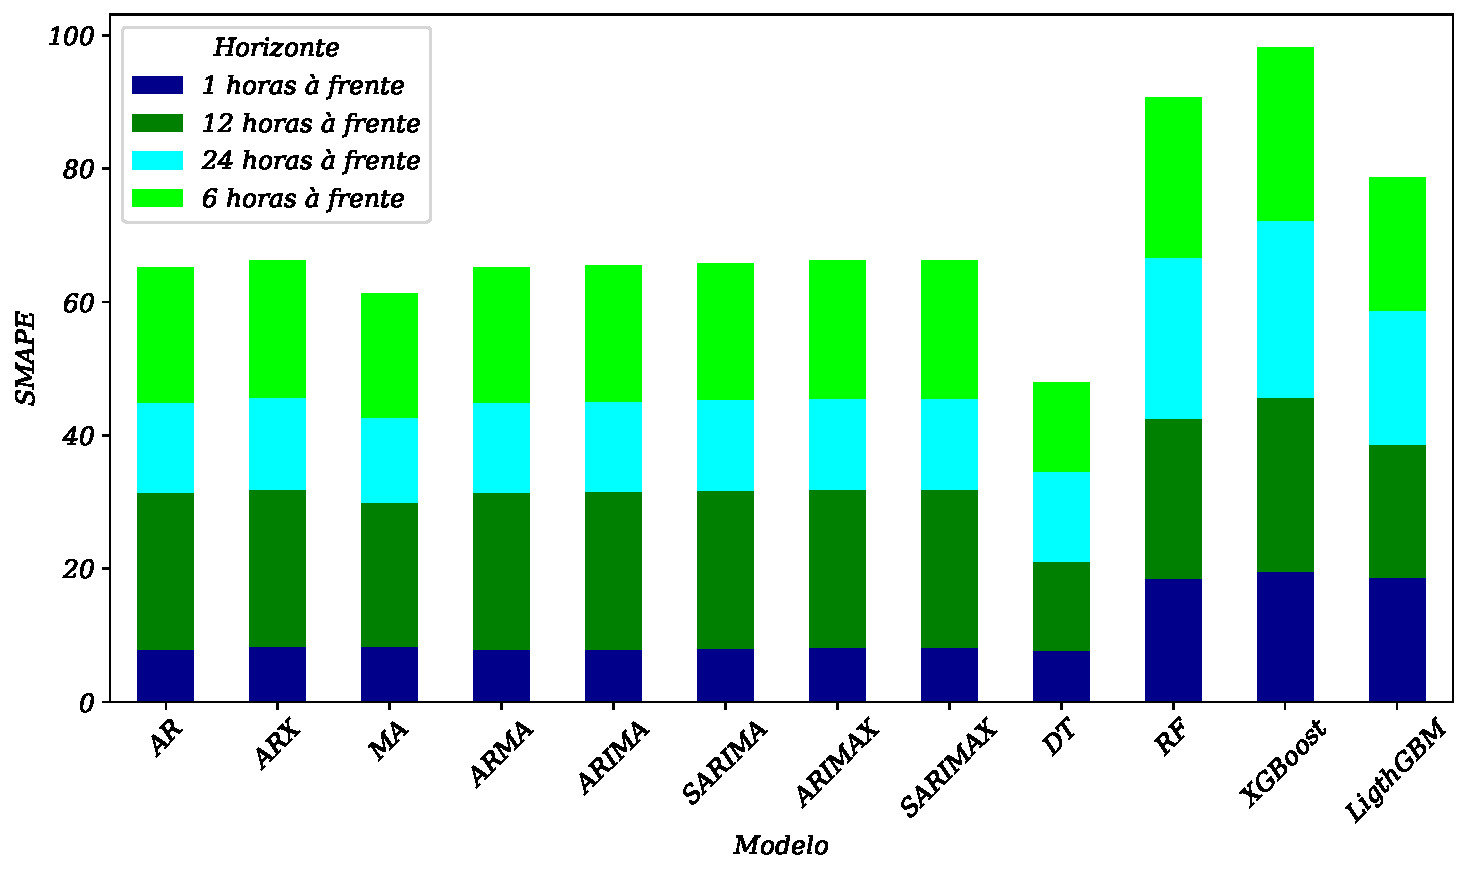
\includegraphics[width=0.7\linewidth]{Resultados/Figuras/smape_comparar_basic}
	
	
\end{figure}

\begin{figure}[H]
	\centering
	\caption{Comparação dos modelos AR, ARX, MA, ARIMA, SARIMA, ARIMAX, SARIMAX, DT, RF, XGBoost, LightGBM em vários horizontes na métrica MAE.}\label{fig:modelos-arima}
	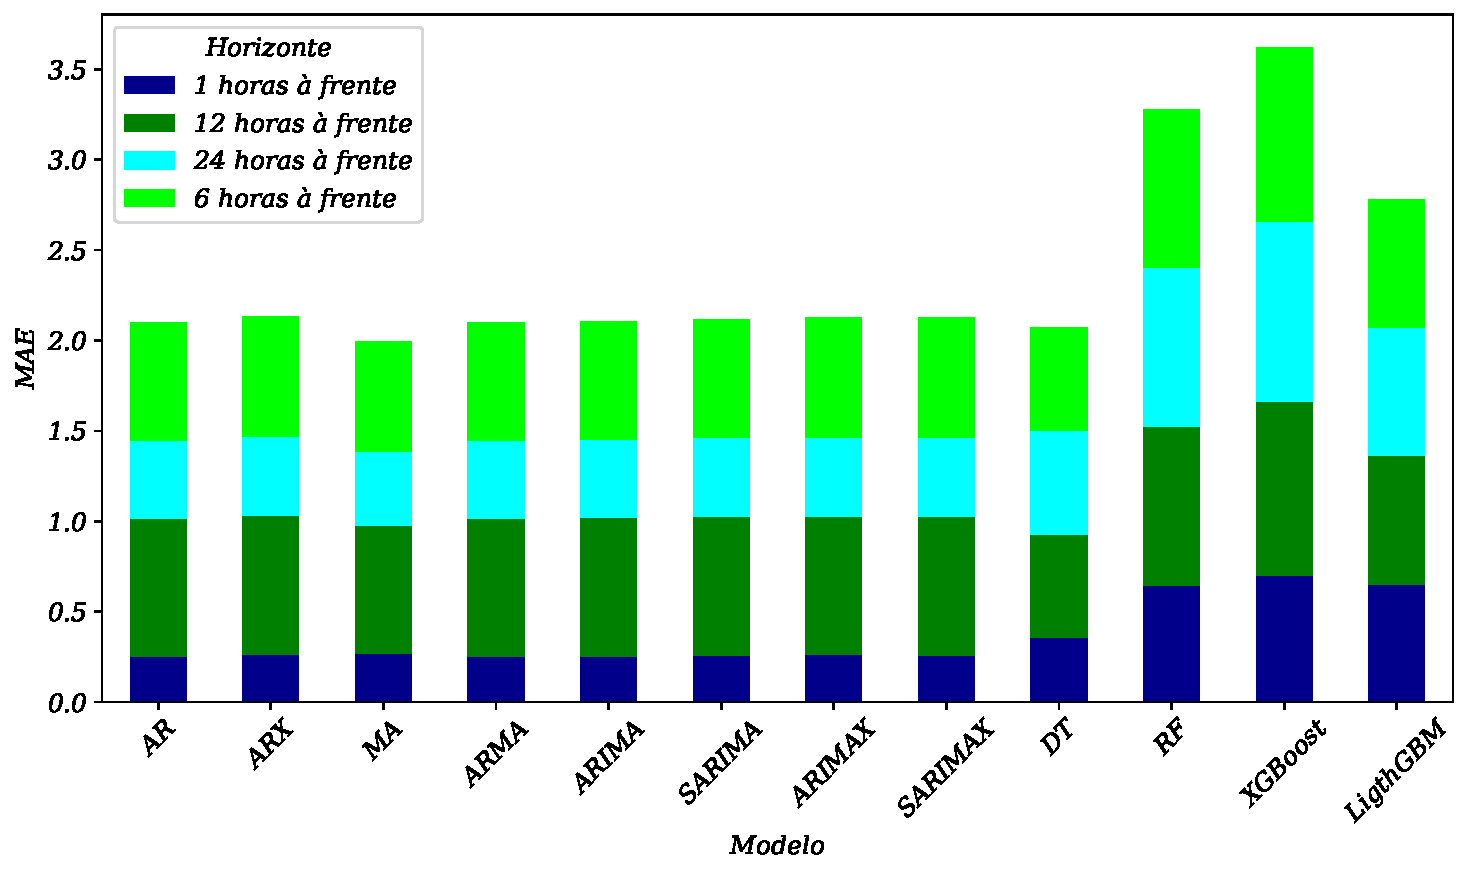
\includegraphics[width=0.7\linewidth]{Resultados/Figuras/mae_comparar_basic}
	
	
\end{figure}

\begin{figure}[H]
	\centering
	\caption{Comparação dos modelos AR, ARX, MA, ARIMA, SARIMA, ARIMAX, SARIMAX, DT, RF, XGBoost, LightGBM em vários horizontes na métrica RRMSE.}\label{fig:modelos-arima2}
	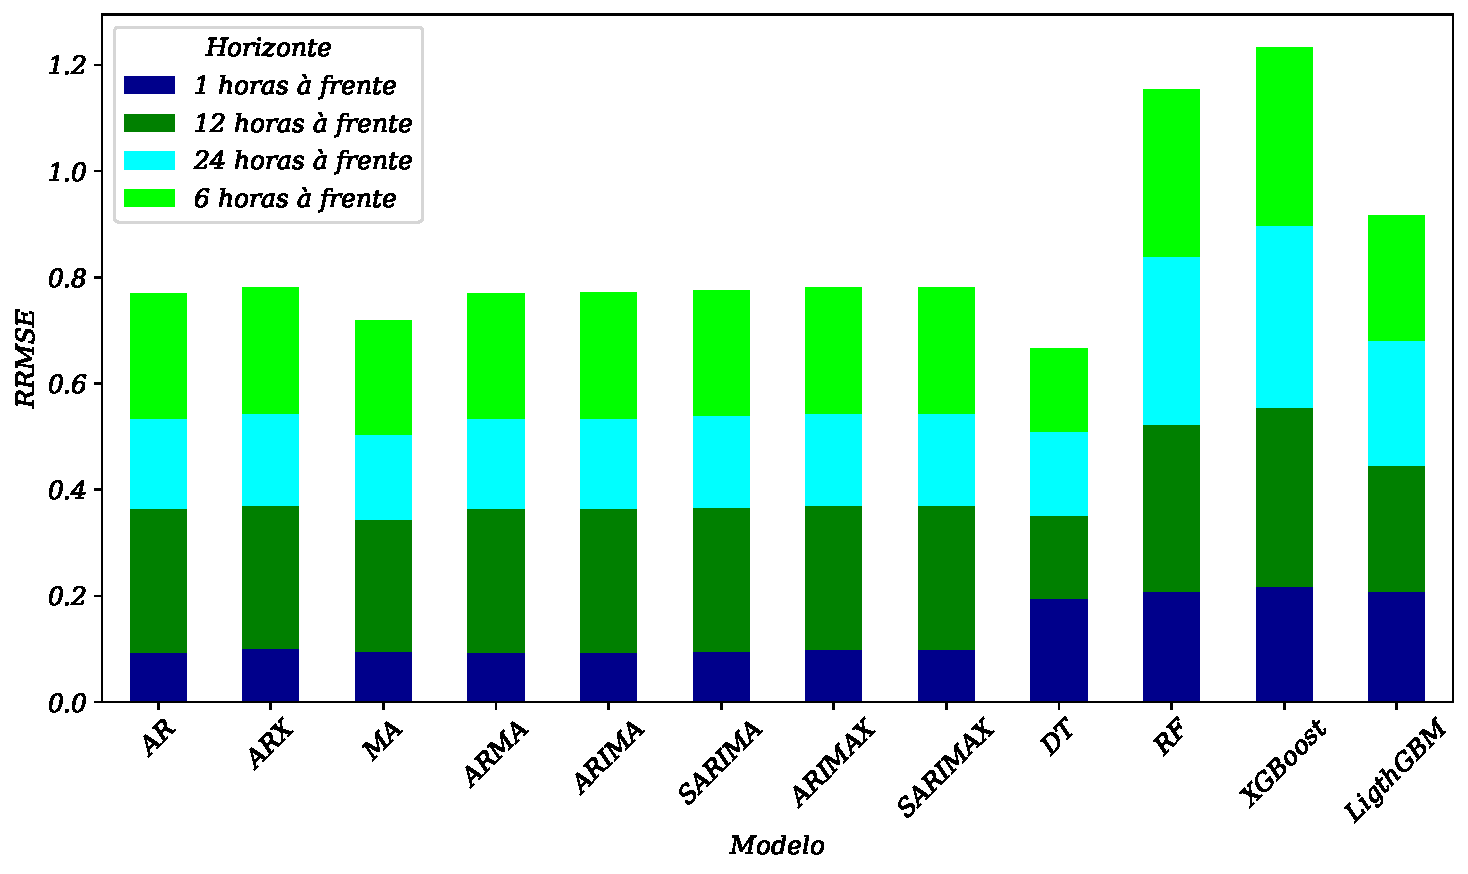
\includegraphics[width=0.7\linewidth]{Resultados/Figuras/rrmse_comparar_basic}
	
	
\end{figure}

\begin{figure}[H]
	\centering
	\caption{Comparação dos modelos Prophet, MLP, CNN, RNN, LSTM, GRU em vários horizontes na métrica SMAPE.}\label{fig:modelos-red1}
	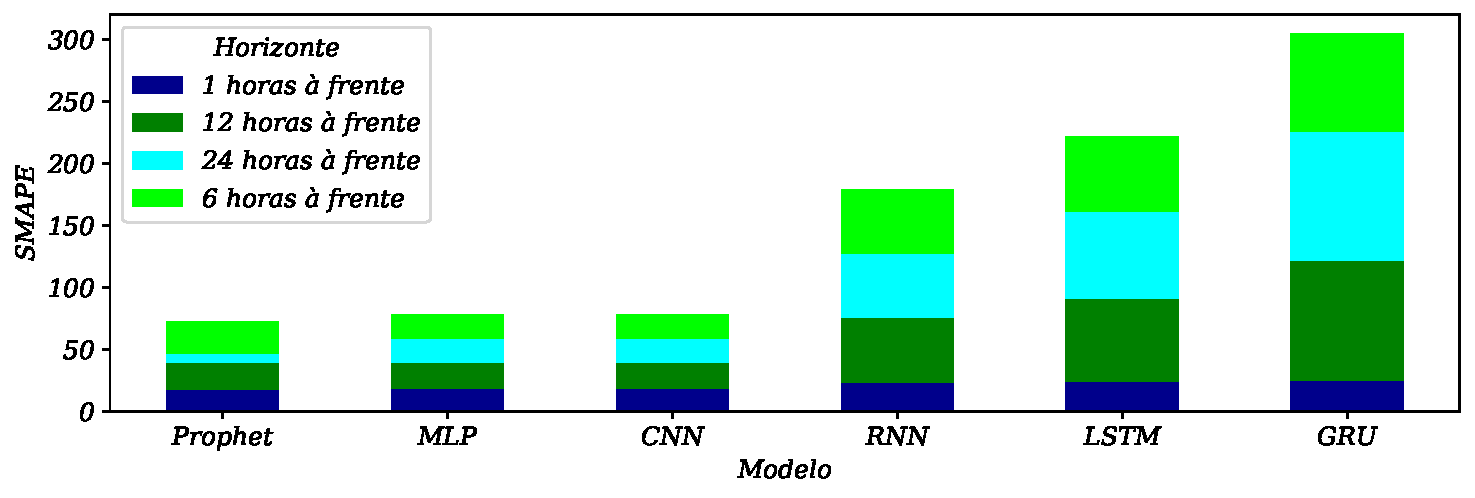
\includegraphics[width=0.9\linewidth]{Resultados/Figuras/smape_comparar}
	
	
\end{figure}



\begin{figure}[H]
	\centering
	\caption{Comparação dos modelos Prophet, MLP, CNN, RNN, LSTM, GRU em vários horizontes na métrica MAE.}\label{fig:modelos-red}
	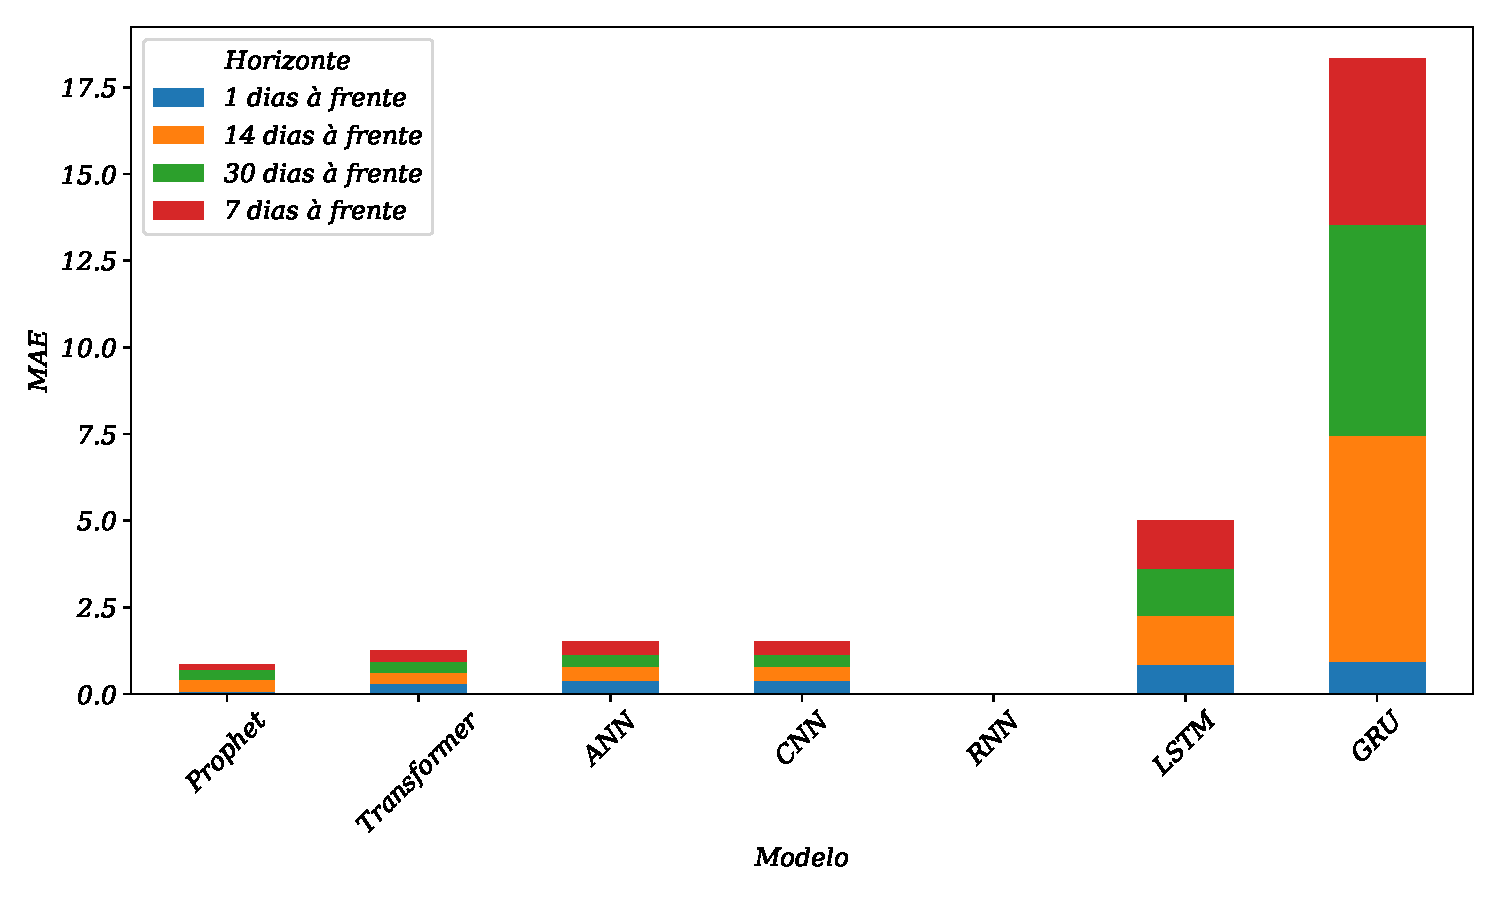
\includegraphics[width=0.9\linewidth]{Resultados/Figuras/mae_comparar}
	
	
\end{figure}



\begin{figure}[H]
	\centering
	\caption{Comparação dos modelos Prophet, MLP, CNN, RNN, LSTM, GRU em vários horizontes na métrica RRMSE.}\label{fig:modelos-red2}
	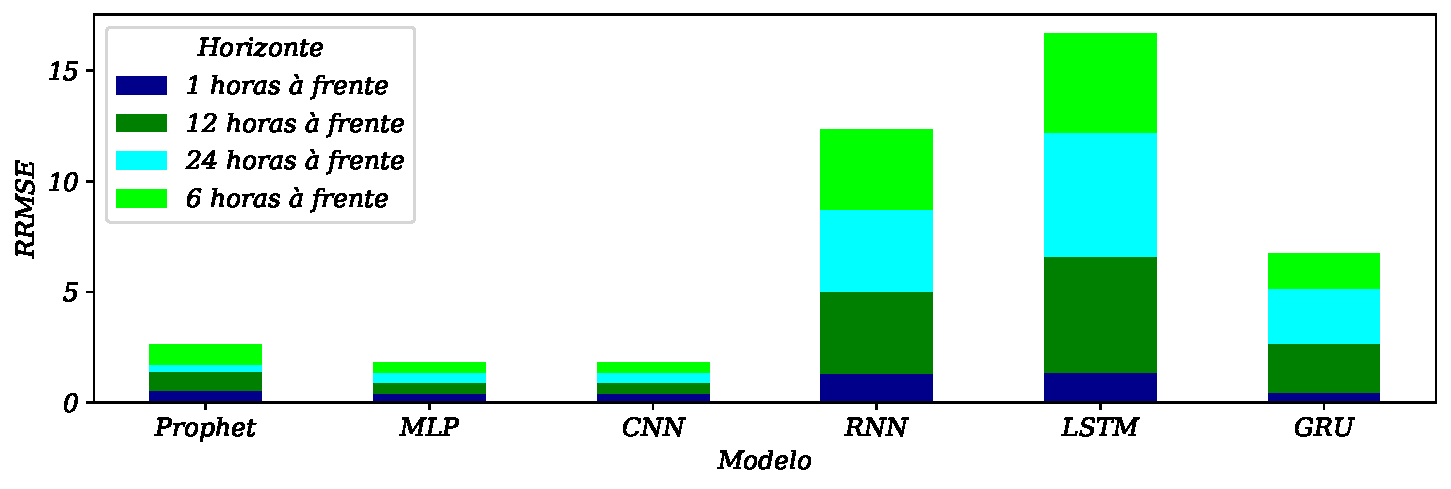
\includegraphics[width=0.9\linewidth]{Resultados/Figuras/rrmse_comparar}
	
	
\end{figure}

A avaliação da eficácia dos modelos ARIMA em previsões de longo prazo emprega o teste de Ljung-Box, conforme detalhado nas Tabelas \ref{tb:lbtrn} a \ref{tb:lbcm} ilustram a acurácia dos modelos ARIMA ao longo do tempo, com valores menores sendo destacados em \textbf{negrito}. Modelos como ARX, ARIMAX e SARIMAX, que incorporam variáveis exógenas, demonstram um desempenho superior nesse contexto. Esses modelos não lineares apresentam uma capacidade de previsão robusta em horizontes temporais mais longos, diferenciando-se positivamente dos outros modelos ARIMA. Nas Figuras \ref{fig:modelos-arima1} a \ref{fig:modelos-arima2}, são selecionados os modelos ARIMA e seus antecessores. Esses modelos têm suas limitações, tanto para horizontes de previsão de curto prazo quanto para horizontes de longo prazo. Esse gráfico pode fornecer várias informações, mas o objetivo aqui é identificar apenas o melhor modelo entre os modelos ARIMA.

Como essa série não apresentou uma estacionariedade bem definida e os dados não a tornaram estacionária, os modelos que não têm sazonalidade mostraram-se superiores, tais como AR, MA, ARX, ARMA, ARIMA e ARIMAX. O modelo ARIMAX demonstrou ser bastante robusto para este caso, mas mesmo assim, modelos mais básicos como AR, ARMA e ARIMA ainda apresentaram resultados melhores.

\begin{table}[H]
	\centering		
	\caption{Comparação dos modelos com o teste Ljung Box modelos ARIMA com defasagem de 10 para previsão de longo prazo na demanda d'água.}
	
	\begin{subtable}{0.49\linewidth}
		\centering
		\caption{\textbf{Treinamento.}} \label{tb:lbtrn}
		\begin{tabular}{@{}lll@{}}
			\toprule
			Ljung  & Estatística  & Valor \\
			Box & de Teste& de p\\\midrule
			ARX & 86,332 & 0           \\
			AR  & 84,118 & 0            \\
			MA  & 87,940 & 0             \\
			ARMA & 26,204 & 0,003         \\
			ARIMA & \textbf{21,4} &\textbf{0,018}  \\
			SARIMA & 97,735 & 0 \\
			ARIMAX & 42,151 & 0   \\
			SARIMAX  & 47,310 & 0                    \\ \bottomrule
		\end{tabular}
	\end{subtable}
	\hfill
	\begin{subtable}{0.49\linewidth}
		\centering
		\caption{\textbf{Validação.}} \label{tb:lbvld}
		\begin{tabular}{@{}lll@{}}
			\toprule
			Ljung  & Estatística  & Valor \\
			Box & de Teste& de p\\\midrule
			ARX       & 6,514                         & 0,770               \\
			AR        & \textbf{0,764}              & \textbf{0,376}     \\
			MA        & 76,952                        & 0                   \\
			ARMA      & 4,900                         & 0,898               \\
			ARIMA     & 11,025                        & 0,356               \\
			SARIMA    & 68,136                        & 0                   \\
			ARIMAX    & 10,809                        & 0,373               \\
			SARIMAX   & 13,287                        & 0                   \\ \bottomrule
		\end{tabular}
	\end{subtable}
			
			\hfill
			
	\begin{subtable}{0.49\linewidth}
		\centering
		\caption{\textbf{Teste.}} \label{tb:lbtst}
		\begin{tabular}{@{}lll@{}}
			\toprule
			Ljung  & Estatística  & Valor \\
			Box & de Teste& de p\\\midrule
			ARX & 36,884 & 0 \\
			AR & 36,799 & 0 \\
			MA & 71,945 & 0 \\
			ARMA & \textbf{9,706} & \textbf{0,467} \\
			ARIMA & 60,289 & 0 \\
			SARIMA & 70,992 & 0 \\
			ARIMAX & 48,435 & 0   \\
			SARIMAX & 45,749 & 0 \\ \bottomrule
		\end{tabular}
	\end{subtable}	
\hfill	
	\begin{subtable}{0.49\linewidth}
		\centering
		\caption{\textbf{Inteiro.}} \label{tb:lbcm}
		\begin{tabular}{@{}lll@{}}
			\toprule
			Ljung  & Estatística  & Valor \\
			Box & de Teste& de p\\\midrule
			ARX       & 22,944                        & 0                   \\
			AR        & \textbf{22,715}               & \textbf{0}          \\
			MA        & 5725,300                      & 0                   \\
			ARMA      & 72,446                        & 0                   \\
			ARIMA     & 72,446                        & 0                   \\
			SARIMA    & 72,446                        & 0                   \\
			ARIMAX    & 84,362                        & 0                   \\
			SARIMAX   & 23,537                        & 0                   \\ \bottomrule
		\end{tabular}
	\end{subtable}
	
	
%	\vspace{0.5cm}
	
\end{table}





